\documentclass[english, aip, jcp, priprint, graphicx]{revtex4-1}
\usepackage{amsmath}
\usepackage{amsthm}
\usepackage{amssymb}
\usepackage{mathrsfs}
\usepackage{bbm,latexsym}
\usepackage{graphicx}

%%%%%%%%%% Start TeXmacs macros
\catcode`\<=\active \def<{
\fontencoding{T1}\selectfont\symbol{60}\fontencoding{\encodingdefault}}
\catcode`\>=\active \def>{
\fontencoding{T1}\selectfont\symbol{62}\fontencoding{\encodingdefault}}
\newcommand{\mathd}{\mathrm{d}}
\newcommand{\nin}{\not\in}
\newcommand{\tmop}[1]{\ensuremath{\operatorname{#1}}}
\newcommand{\tmtextbf}[1]{{\bfseries{#1}}}
\newtheorem{definition}{Definition}
\newtheorem{proposition}{Proposition}
\newtheorem{theorem}{Theorem}
\newtheorem{lemma}{Lemma}
\newtheorem{algorithm}{Algorithm}
%%%%%%%%%% End TeXmacs macros

\draft % marks overfull lines with a black rule on the right

\theoremstyle{plain}
\newtheorem{thm}{\protect\theoremname}
\theoremstyle{definition}
\newtheorem{defn}[thm]{\protect\definitionname}
\theoremstyle{plain}
\newtheorem{cor}[thm]{\protect\corollaryname}

\usepackage{babel}
\providecommand{\corollaryname}{Corollary}
\providecommand{\definitionname}{Definition}
\providecommand{\lemmaname}{Lemma}
\providecommand{\theoremname}{Theorem}

\begin{document}

\title{Overcoming Entropic Barriers by Capacity Hopping} %Title of paper

\author{Jackson Loper}
\thanks{These two authors contributed equally}
\affiliation{Data Science Institute, Columbia University, New York, NY, USA}

\author{Guangyao Zhou}
\thanks{These two authors contributed equally}

\author{Stuart Geman}

\affiliation{Division of Applied Mathematics, Brown University, Providence, RI, USA}
\date{\today}

\begin{abstract}
	We show how to accelerate molecular dynamics simulations using theoretical analysis of large regions in the configuration space with flat energy landscape. Due to entropic effects, a system may spend significant time in these large, flat regions, just as enthalpic effects may cause a system to spend significant time trapped in local energetic minima.  Many advances have been made in the theoretical analysis of local minima, but there has been little study of large, flat regions. Experimental evidence suggests that these regions are ubiquitous in biomolecular systems, and often characterize the rate-limiting step of biomolecular processes.  In this paper, we investigate the probabilities of entering various target sets inside these flat regions. We show that these flat regions are characterized by \emph{approximately constant hitting probabilities} for the target sets, and connect these hitting probabilities to \textit{capacities} of local sets around the targets.  Using these theoretical results and a new capacity estimation algorithm, we develop Capacity Hopping (CHop), a method for accelerating molecular dynamics simulations. Numerical experiments on a toy model with a golf-course potential show that CHop is nearly as accurate as naive simulations in estimating hitting probabilities, but 750 times faster.
\end{abstract}

\pacs{}% insert suggested PACS numbers in braces on next line

\maketitle %\maketitle must follow title, authors, abstract and \pacs

\global\long\def\capac#1#2{\mathrm{cap}\left(#1;#2\right)}
\global\long\def\fnsp{\mathscr{H}^1}
\global\long\def\bb#1{\mathcal{B}\left(#1\right)}

\section{Introduction}
Molecular dynamics, first introduced in the 1970s \cite{McCammon1977-kg, Warshel1976-qg}, has evolved into an indispensable tool in the study of structures and functions of macromolecules, and allows us to obtain a detailed understanding of the dynamics of a diverse range of biomolecular processes, including the folding of macromolecules into their native configurations \cite{Scheraga2007-qw}, and the conformational changes involved in their functioning \cite{Hospital2015-ol}.

Yet despite the substantial increase in speed and accuracy of molecular dynamics simulations over the years, we are still severely limited in the timescale we can access. Even with specialized hardwares, we can only achieve atomic-level simulations on timescales as long as milliseconds\cite{Dror2012-ws}, while the timescales for various biomolecular processes vary widely, and can last for seconds or longer\cite{Naganathan2005-ki, Zemora2010-lb}. The challenges of molecular dynamics result from the complicated energy landscapes associated with different biomolecular systems, and can be summarized by two main difficulties: the difficulty of escaping local minima (the ``enthalpic" effects), and the difficulty of reaching a small number of target configurations out of a vast number of possible configurations (the ``entropic" effects).

Great efforts have been put into extending the timescale accessible by molecular dynamics simulations. A lot of methods focus on enhanced sampling, with simulated annealing \cite{Kirkpatrick1983-su}, genetic algorithms\cite{Goldberg1989-ko} and parallel tempering\cite{Sugita1999-vh} as representatives. However, dynamics is destroyed in these methods, and additional work\cite{Yang2007-gn, Andrec2005-fh, Zheng2009-ow, Huang2010-uu} is needed in order to recover the kinetic information of the system, usually under the framework of kinetic transition networks\cite{Noe2006-cs, Wales2006-ur} or Markov State Models \cite{Pande2010-yi, Chodera2014-bh, Husic2018-xp}. When focusing directly on kinetics, the foundational work is transition state theory\cite{Eyring1935-ur, Chandler1978-bq, Wigner1997-kk}. Various other methods build on top of this, including  transition path sampling\cite{Dellago1998-lb, Bolhuis2002-ws}, transition interface sampling\cite{Van_Erp2005-vw}, and the more recent transition path theory\cite{E2006-fm, E2010-sr}. The essential idea here is to provide information about the reaction rates between different states, which can then be used under the framework of kinetic transition networks\cite{Noe2006-cs, Wales2006-ur} or Markov State Models \cite{Pande2010-yi, Chodera2014-bh, Husic2018-xp} to understand the kinetics of the system. In addition, different accelerated molecular dynamics methods\cite{Perez2009-jy}(hyperdynamics\cite{Voter1997-gi}, parallel replica\cite{Voter1998-mv} and temperature-accelerated dynamics\cite{Sorensen2000-qm}) aim at directly accelerating the molecular dynamics simulations, by either smoothing the energy landscape, exploring energy basins in parallel, or raising the temperature while maintaining the correct dynamics. We refer the readers to some other reviews\cite{Klenin2011-jf, Christen2008-ge, Perez2009-jy} for a more comprehensive picture of this area.

Careful inspection of the existing methods shows that a majority of the previous developments focus on the enthalpic effects, where the central picture consists of an energy landscape with a multitude of local minima separated by high energetic barriers.  A less studied picture involves the entropic effects.  Even when the energy landscapes has essentially no local minima, the dynamics can still be quite complex \cite{Baum1986-we, Wille1987-tf}.  Some efforts have been made to analyze these kinds of systems \cite{Reguera2001-qa, Lwin2005-dm, Mondal2010-oh, Huang2009-kc, Sorensen2000-qm}, but existing work focuses primarily on ``bottleneck" models, where two large regions are connected by a small channel.  In this paper we focus on ``golf-course" potentials: a large flat region with several small targets on it. The importance of this golf course picture lies in its ubiquity in biomolecular systems, and its role in characterizing the rate-limiting step for a variety of processes, as demonstrated by strong experimental  evidence \cite{Teschner1987-qs, Jacob1999-bs, Goldberg1999-mv, Plaxco1998-iv} that ``folding rates are controlled by the rate of diffusion of pieces of the open coil in their search for favorable contacts"\cite{McLeish2005-dq}. In fact, ``the vast majority of the space covered by the energy landscape must actually be flat"\cite{McLeish2005-dq}, indicating the presence and significance of entropic effects.  The difficulty for dealing with entropic effects has been identified in various places. In previous works\cite{Baum1986-we, Wille1987-tf, Machta2009-gh}, it's pointed out that enhanced sampling methods such as simulated annealing and parallel tempering work poorly in the presence of entropic effects. In accelerated molecular dynamics\cite{Sorensen2000-qm}, the authors refer to this problem as the ``low barrier problem". In the review \cite{Christen2008-ge}, the author takes a largely pessimistic view on this subject: ``If these processes are intrinsically slow, i.e. require an extensive sampling of state space'' (which is indeed the case in the presence of entropic effects), ``not much can be done to speed up their simulation without destroying the dynamics of the system.''

In this paper, we argue for a new point of view: for molecular dynamics simulations, the intrinsic slowness and long timescales involved in golf-course potentials can be a blessing rather than a curse.  Indeed, if the targets are sufficiently small and the potential energy is sufficiently flat, the system must reach a local equilibrium before it hits one of the targets. In this case, the starting point becomes irrelevant. Thus, if a region has a golf course potential, the hitting probabilities are nearly constant for nearly all of the region. It turns out these probabilities can be approximated using only local information from the vicinities of the targets, coming in the form of “capacities.”   Whenever the dynamics lead out into a flat region of the potential, we can thus simply hop directly to a target, randomly chosen according to the correct probabilities.  This allows us to accelerate simulations by skipping over the time spent in the flat regions.

The contributions of this paper are twofold:

\begin{description}
	\item[Theory] We present new theoretical results about regions with golf-course potentials.  We show that these regions are characterized by approximately constant hitting probabilities.  We then demonstrate that these probabilities can be approximated using the so-called “capacities” of local sets around the targets.
	\item[Application] Inspired by the theoretical results, we present CHop as a general method to accelerate molecular dynamics simulation, and further propose an efficient capacity estimation algorithm to address the central computational issue of CHop.  We verify the effectiveness of CHop through extensive numerical experiments.
\end{description}

The rest of the paper is organized as follows. In Section \ref{sec:toy_model}, we present a toy model with a golf-course potential.  This example will run across the entire paper as a central thread for our theoretical and numerical analysis. In Section \ref{sec:model_formulation}, we present our theoretical results. We propose the concept of $\varepsilon$-flatness to capture the idea that hitting probabilities remain approximately a constant, and establish the $\varepsilon$-flatness of the toy model in Theorem \ref{thm:epsilon_flat}. We make further connections of the global hitting probabilities to capacities of local sets around the targets in Corollary \ref{thm:main_cor}, for general stationary reversible SDEs. In Section \ref{sec:algorithm}, we talk about applications. We propose CHop as a general method for accelerating molecular dynamics simulations, and discuss the central computational issue of CHop: the efficient estimation of the capacities. We present extensive numerical experiments and results in Section \ref{sec:experiments} to demonstrate the effectiveness of CHop, before giving conclusions and future directions in Section \ref{sec:conclusion}.

\section{A Toy Model}\label{sec:toy_model}

To concretely demonstrate the CHop method, we introduce a simple toy model with a golf-course potential. The potential energy landscape is flat, except for the regions around the two targets $A$ and $B$. This large flat region demonstrates the entropic effects -- the sheer size of it means that it would take the process a long time to find either $A$ or $B$, even though there is no local energetic minima away from $A$ or $B$. To further simplify the analysis and facilitate numerical validation, we will assume all sets of interest are spheres.  A sketch of the relevant sets may be seen in Figure \ref{fig:golfsets}.

\begin{figure}
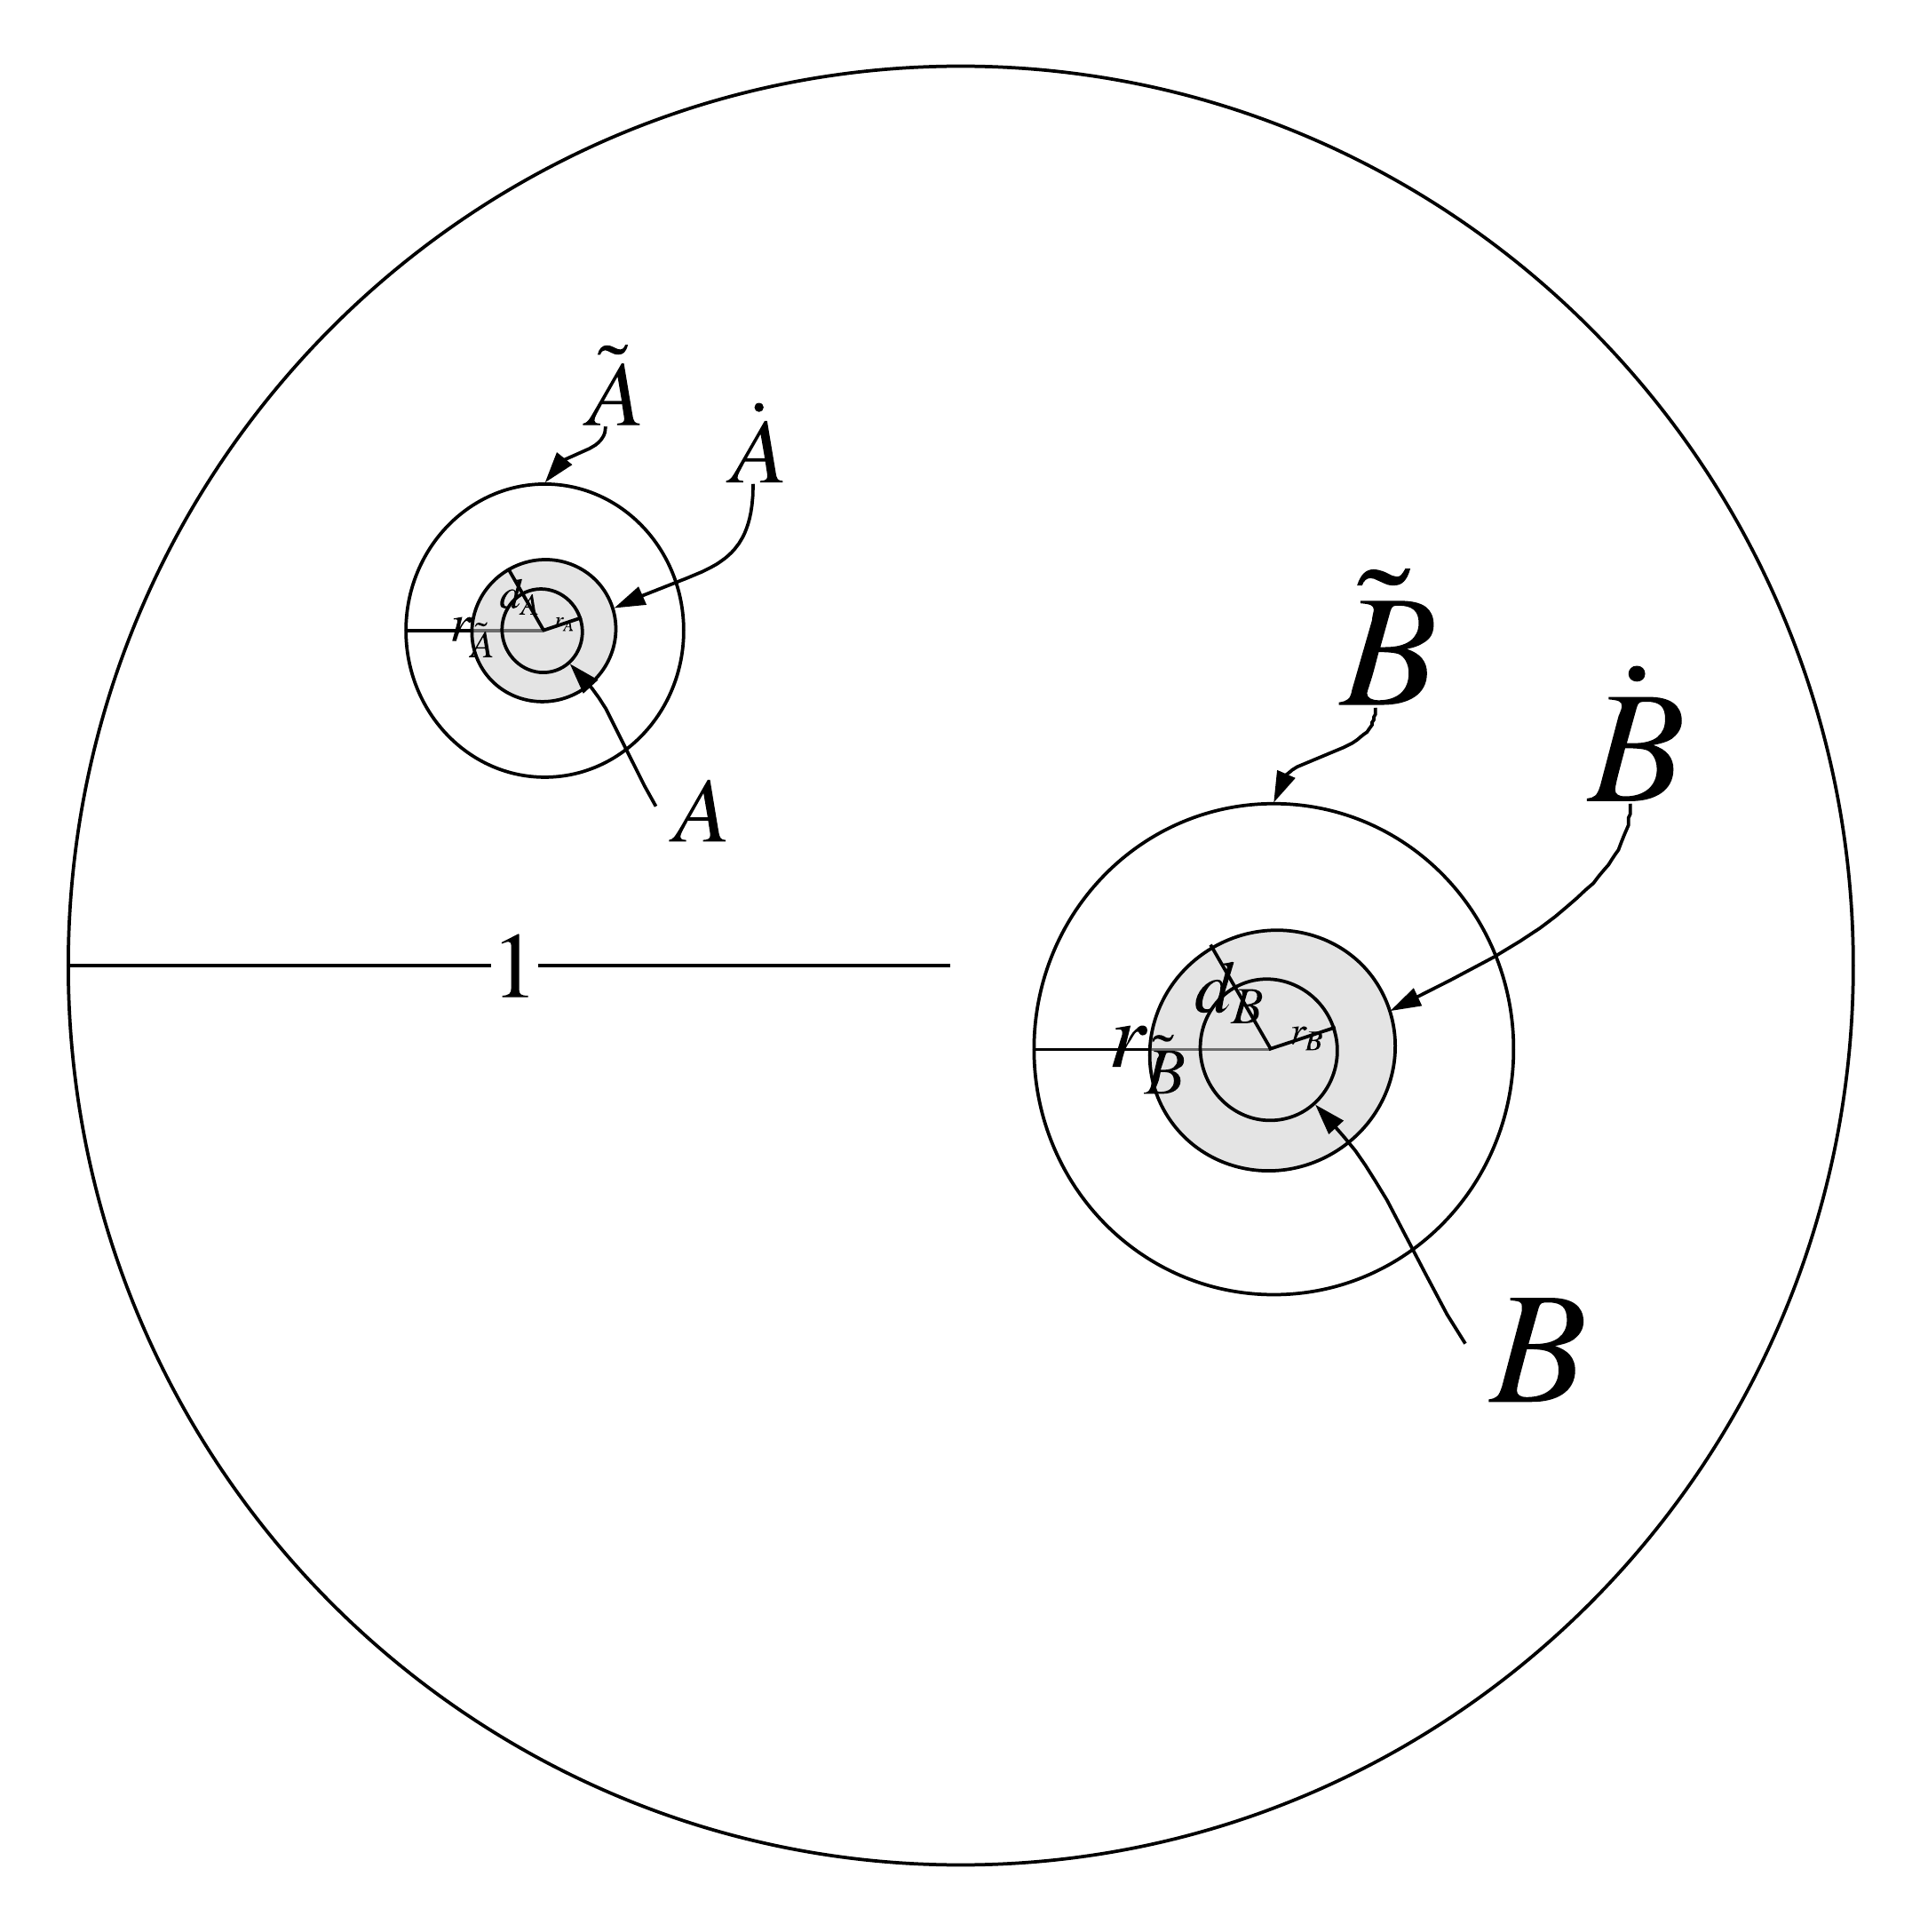
\includegraphics[width=.5\textheight]{figs/golfpic}
\caption{\label{fig:golfsets} The sets and distances involved on the toy model.}
\end{figure}

Formally, denote the ball of radius $r$ centered at a point $x \in \mathbbm{R}^d$ by 
\begin{equation*}
\bb{x, r} = \{ y : || y - x || \leqslant r \}
\end{equation*}
Assume we have $x_A , x_B \in \Omega=\bb{0, 1} \subset \mathbbm{R}^d$ and $0 < r_A < d_A < r_{\tilde{A}}, 0 < r_B < d_B < r_{\tilde{B}}$ such that
\begin{equation*}
r_{\tilde{A}} + \| x_A \| < 1, r_{\tilde{B}} + \| x_B \| < 1, \bb {x_A, r_{\tilde{A}}} \cap \bb {x_B, r_{\tilde{B}}} = \varnothing
\end{equation*}
Define
\begin{align*}
A &= \bb {x_A, r_A}, \dot{A} = \bb {x_A, d_A}, \tilde{A} = \bb {x_A, r_{\tilde{A}}}\\
B &= \bb {x_B, r_B}, \dot{B} = \bb {x_B, d_B}, \tilde{B} = \bb {x_B, r_{\tilde{B}}} 
\end{align*}
Our toy model is governed by the SDE
\begin{equation} \label{equ:toy_sde}
\mathrm{d} X_t = - \nabla U (X_t) \mathrm{d} t + \mathrm{d} W_t 
\end{equation}
with reflecting boundary at $\partial \bb {0, 1}$, where $U$ is a continuous potential function for which $U (x) = 0, \forall x \not\in \dot{A} \cup \dot{B}$, and $W_t$ is the $d$-dimensional Brownian motion. In other words, the toy model follows a diffusion process within $\bb {0, 1}$ with trivial potential energy outside the set $\dot{A} \cup \dot{B}$, and trivial diffusion coefficients. Given an initial configuration, $X_0 = x$, we will be interested to know the probability that the diffusion hits $A=\bb{x_A,r_A}$ before it hits $B=\bb{x_B, r_B}$.

This toy model encapsulates the essential characteristics of entropic effects: if $r_A, r_B$ are small, the trajectory of $X$ will generally be spent well away from $A$ or $B$, in the large flat region of the energy landscape that separates $A$ from $B$. The nontrivial energy landscapes in the immediate vicinity of $A$ and $B$ reflect the local nature of energetic interactions in the system under biological conditions, and the reflecting boundary $\partial\Omega$ captures the notion that not all configurations for the biomolecular system are sensible, because of, for example, the limits on bond lengths, angles and dihedral angles in the case of RNA molecules.

\section{Theory: $\varepsilon$-flatness and CHop Probabilities}\label{sec:model_formulation}

With this toy model in mind, we now turn to the general results of this paper. Assume the underlying physical process $\{X_t\}_{t \geqslant
0}$ that's governing the macromolecule is a stationary reversible diffusion process in the configuration space $\Omega$ with invariant
measure ${\mu}= e^{- U (x)} \mathrm{d} x$, and its dynamics can be described by the SDE
\begin{equation}\label{equ:general_sde}\mathrm{d} X_t = b (X_t) \mathrm{d} t + \sigma (X_t) \mathrm{d} W_t \end{equation}
where $b (\cdot) : \Omega \rightarrow \mathbbm{R}^d$ and $\sigma (\cdot) :
\Omega \rightarrow \mathbbm{R}^{d \times m}$ are differentiable vector-valued
and matrix-valued functions, and $W_t$ is the $m$-dimensional Brownian motion. We refer the reader to Appendix \ref{sec:reversible_diffusion} for a detailed account of stationary reversible diffusion processes.

Let $ \tau_S = \inf \{ t \geqslant 0 : X_t \in S \}, \forall S \subset \mathbbm{R}^d $ denote the time at which the process $\{X_t\}_{t \geq 0}$ first hits set $S$. For fixed target sets $A$ and $B$, we care about hitting probabilities of the form 
\[ h_{A, B}(x) = \mathbb{P}(X_{\tau_{A\cup B}}\in A|X_0=x), \forall x\in \Omega\]
i.e. the probability that $\{X_t\}_{t \geq 0}$ hits $A$ before $B$ given that it starts at $x\in\Omega$. 

Our basic intuition is that, if $A$ and $B$ are sufficiently small relative to $\Omega$, and $U$ is sufficiently flat in $\Omega / (A\cup B)$, then for any starting point $x\in \Omega / (A\cup B)$ away from the target sets $A$ and $B$, we would reach local equilibrium before we hit the targets, and the hitting probability $h_{A, B}(x)$ remains approximately a constant. In addition, since we reach local equilibrium before we hit the targets, the internal structure of $\Omega / (A\cup B)$ away from $A$ and $B$ doesn't matter, and we expect the approximately constant hitting probability $h_{A, B}(x)$ can be accurately estimated using only local information around the targets $A$ and $B$.

In what follows, we make the above intuitions rigorous: we first establish approximately constant hitting probability in the context of our toy model, and then present a theorem showing the connection between the approximately constant hitting probability and the ``capacities" of local sets around the targets.

\subsection{Approximately Constant Hitting Probability}

In this section, we introduce the concept of $\varepsilon$-flatness, and establish it for our toy model, to capture the notion that the hitting probability $h_{A, B}(x)$ remains approximately a constant in $\Omega / (A\cup B)$ away from $A$ and $B$, when $A$ and $B$ are sufficiently small relative to $\Omega$, and $U$ is sufficiently flat on $\Omega / (A\cup B)$.

\begin{definition}($\varepsilon$-flatness)\label{def:epsilon_flat}
For any function $u$ on $\Omega$ and an $\varepsilon > 0$, a set $M\subset \Omega$ is $\varepsilon$-flat for the function $u$ if $\sup_{x, y \in M} | u (x) - u (y) | < \varepsilon$.
\end{definition}

Armed with this definition, we present a theorem in the context our toy model, which establishes the $\varepsilon$-flatness of the set $\bb {0, 1} / (\tilde{A} \cup \tilde{B})$ for the hitting probability $h_{A, B}(x)$, when the targets $A, B$ are sufficiently small or the dimension is high, for suitably picked sets $\tilde{A}, \tilde{B}$.

\begin{theorem}\label{thm:epsilon_flat}
Let $u\triangleq h_{A, B}$, where the diffusion and $A, B$ are defined by the toy model given in Equation \ref{equ:toy_sde} parametrized by $x_A, x_B, r_A, d_A, r_{\tilde{A}}, r_B, d_B, r_{\tilde{B}}$. For any fixed value of $d \geq 3$ and $r_{\tilde{A}}, r_{\tilde{B}}, \varepsilon > 0$, there exists a constant $c=c(d, r_{\tilde{A}}, r_{\tilde{B}}, \varepsilon)$ such that if $d_{A}, d_{B} < c$ then
\begin{equation*}
	\sup_{x, y \in \bb {0, 1} / (\tilde{A} \cup \tilde{B})}|u(x)-u(y)| < \varepsilon
\end{equation*}
Likeliwise for any fixed value of $d_{A}, r_{\tilde{A}}, d_{B}, r_{\tilde{B}}, \varepsilon>0$, there exists a constant $c=c(d_{A}, r_{\tilde{A}}, d_{B}, r_{\tilde{B}}, \varepsilon)$ such that if $d \geq c$ then the same holds.
\end{theorem}

We defer the proof of this theorem to Appendix \ref{sec:proof_epsilon_flat}. Inspection of the proof demonstrates that the key for establishing $\varepsilon$-flatness is a proper separation of time scales: it takes a short time for the process $\{X_t\}_{t\geq 0}$to reach local equilibrium in $\bb {0, 1} / (\tilde{A} \cup \tilde{B})$, because of the flatness of the potential energy $U$ in this set, while it takes a long time for the process $\{X_t\}_{t\geq 0}$ to hit the targets $A$ and $B$, starting in $\bb {0, 1} / (\tilde{A} \cup \tilde{B})$, because of the sizes of the targets $A$ and $B$ being small compared with $\Omega$.

\subsection{Estimating Constant Hitting Probability Using Local Information}

In this section, we present results showing that when $\varepsilon$-flatness is established, we can accurately estimate the approximately constant hitting probability $h_{A, B}(x)$ using only local information around the targets. It turns out this local information comes in the form of capacities of sets around the targets. For $A \subset \tilde{A} \subset \Omega$, the capacity
$\ensuremath{\operatorname{cap}} (A, \tilde{A})$ under the stationary reversible diffusion process $\{X_t\}_{t\geq 0}$ is given by
\[ \ensuremath{\operatorname{cap}} (A, \tilde{A}) = \frac{1}{2} \int_{\Omega}
\nabla h_{A, \tilde{A}^c} (x)^T a (x) \nabla h_{A, \tilde{A}^c} (x) e^{- U
(x)} \mathrm{d} x \]
where $a (x) = \sigma (x) \sigma (x)^T$ is the diffusion matrix. We refer the reader to Appendix \ref{sec:reversible_diffusion} for more details on capacity and the the related concept of Dirichlet form.

We start by considering the simple case where there are only two targets $A$ and $B$. For the general stationary reversible SDE given by Equation \ref{equ:general_sde}, we have our main theorem

\begin{theorem}\label{thm:main_thm}
Assume we have $A, B \subset \Omega$ disjoint. Define
\[ u (x) = h_{A, B}(x) = \mathbbm{P} (X_{\tau_{A \cup B}} \in A|X_0 = x) \]
$\forall \varepsilon \in \left( 0, \frac{2}{9} \right]$, if we can find
$\tilde{A}, \tilde{B} \subset \Omega$, s.t. $A \subset \tilde{A}, B \subset
\tilde{B}$, and $M = \Omega / (\tilde{A} \cup \tilde{B})$ is $\varepsilon$-flat
for the function $u$, then we have
\[ \sup_{x \in M} \left| u (x) - \frac{\ensuremath{\operatorname{cap}} (A,
\tilde{A})}{\ensuremath{\operatorname{cap}} (A, \tilde{A})
+\ensuremath{\operatorname{cap}} (B, \tilde{B})} \right| \leqslant
\varepsilon + \sqrt{\frac{\varepsilon}{2}} \]
\end{theorem}

We defer the proof to Appendix \ref{sec:proof_thm}. This theorem generalizes naturally to the case of multiple targets, with the additional definition of \textit{CHop Probabilities}:

\begin{definition}\label{chop_prob}
Let $\{X_t\}_{t\geq 0}$ be a stationary reversible diffusion process on $\Omega$.  Pick $A_1\cdots A_n \subset \Omega$ and $\tilde A_1\cdots \tilde A_n \subset \Omega$ such that $A_k \subset \tilde A_k$.  Then the \textbf{CHop Probability} for the set $A_k$ (given all the other sets $A_1\cdots, A_{k-1}, A_{k+1}, \cdots A_n \subset \Omega$ and $\tilde A_1\cdots \tilde A_n \subset \Omega$) is given by
\begin{equation*}
p_{A_k} = \frac{\ensuremath{\operatorname{cap}} (A_k, \tilde{A}_k)}{\sum_{i = 1}^n \ensuremath{\operatorname{cap}} (A_i, \tilde{A}_i)}, k=1,\dots, n
\end{equation*} 
\end{definition}

\begin{cor}\label{thm:main_cor} Let $u_k = h_{A_k,\cup_{i\neq k} A_i}$ denote the probability the process hits $A_k$ before the other target sets.  Fix any $\varepsilon \in \left( 0, \frac{2}{9} \right]$.  If $M = \Omega \backslash \bigcup_{k = 1}^n \tilde{A}_k $ is $\varepsilon$-flat for the functions $\{u_k\}_{k\in1,\dots, n}$ then each $u_k$ is well-approximated by the corresponding CHop Probability:
\[ \sup_{x \in M} \left| u_k (x) - p_{A_k} \right| \leqslant \varepsilon + \sqrt{\frac{\varepsilon}{2}}, k=1,\dots, n\]
\end{cor}

This corollary follows immediately from Theorem \ref{thm:main_thm} and additivity of the capacity (Proposition \ref{prop:capacity} in Appendix \ref{sec:reversible_diffusion}). 

\section{Application: CHop Method and Capacity Estimation}\label{sec:algorithm}

In this section, we focus on practical applications. Inspired by the theoretical analysis above, we introduce the CHop method as a way to accelerate molecular dynamics simulations by efficiently dealing with regions with golf-course potential. We present the high-level idea of the CHop method, and give a detailed account of the key computational issue of the CHop method, the efficient estimation of capacities. A general framework based on a simple lemma is given for capacity estimation, and the associated challenges are discussed. To demonstrate this framework, we give an outline of a flexible and general-purpose algorithm for capacity estimation, and make some concrete choices to show how exactly the algorithm works in the case of our toy model. This will serve as the basis for the numerical experiments and results in Section \ref{sec:experiments}.

\subsection{CHop Method}

Recall that in the previous section on theory, we made the following two key points:

\begin{enumerate}
	\item We can establish $\varepsilon$-flatness in regions with a golf-course potential, and the hitting probabilities of the various targets remains approximately a constant over a large part of the flat region.
	\item The approximately constant hitting probabilities can be accurately estimated using CHop probabilities, which depend on capacities that can be determined solely based on the local information around the targets.
\end{enumerate}

In most practical applications, molecular dynamics simulations of biomolecular systems are not fast enough to give us information on a biologically relevant time-scale. A large part of this difficulty results from golf-course potentials\cite{Teschner1987-qs, Jacob1999-bs, Goldberg1999-mv, Plaxco1998-iv, McLeish2005-dq}. The above theoretical insights provide us with an efficient way to deal with golf-course potentials, so that we can get information of the biomolecular system on a much longer time-scale: we make use of our knowledge of the targets (which is typically available, e.g. in the form of different secondary structures for RNAs) to carry out local simulations around the targets for the estimation of capacites. Capacities can then be used to calculate the CHop probabilities, which give us an accurate estimate of the approximately constant hitting probabilities. This enables us to make probabilistic jumps to one of the targets to accelerate the molecular dynamics simulations, which is the essence of the CHop method.

To summarize, the CHop method works with a region $\Omega$ which has a golf-course potential under the process $\{X_t\}_{t \geq 0}$. Following the notations in Definition \ref{chop_prob}, we use $A_1\cdots A_n \subset \Omega$ to denote the target sets in the golf-course potential. On a high-level, the CHop method consists of the following steps:

\begin{enumerate}
	\item Identify suitable sets $\tilde A_k \subset \Omega$ where $A_k \subset \tilde{A}_k, k=1, \cdots, n$, such that we can establish the $\varepsilon$-flatness of $M = \Omega \backslash \bigcup_{k = 1}^n \tilde{A}_k $ for hitting probability functions $h_{A_k,\cup_{i\neq k} A_i}(x)$.
	\item Estimate the capacities $\ensuremath{\operatorname{cap}} (A_k, \tilde{A}_k)$, from which we can derive the CHop probabilities
\begin{equation*}
p_{A_k} = \frac{\ensuremath{\operatorname{cap}} (A_k, \tilde{A}_k)}{\sum_{i = 1}^n \ensuremath{\operatorname{cap}} (A_i, \tilde{A}_i)}, k=1,\dots, n
\end{equation*} 
	\item Once the process $\{X_t\}_{t \geq 0}$ enters the flat region $M$, make probabilistic jumps to one of the target sets $A_k$ using the CHop probabilities $p_{A_k}, k=1, \cdots, n$.
\end{enumerate}

It's easy to see that, to make the CHop method practical, we need to be able to estimate the capacities accurately and efficiently. This would be our topic for the rest of this section.

\subsection{Estimation of Capacities}

We start our discussion on estimating the capacities with a simple lemma:
\begin{lemma}\label{thm:capacity_lemma}
For a stationary reversible  diffusion process $X_t$ in $\Omega$ with
invariant measure ${\mu}= e^{- U (x)} \mathrm{d} x$ and diffusion matrix
$a (x)$, given non-empty sets $A \subset G \subset \tilde{G} \subset
\tilde{A}$ with smooth boundaries, the capacity
$\ensuremath{\operatorname{cap}} (A, \tilde{A})$ can be calculated by
\begin{eqnarray*}
\ensuremath{\operatorname{cap}} (A, \tilde{A}) & = & \int_{\partial
\tilde{G}}  h_{A,
\tilde{A}^c} (x) e^{- U (x)} [a (x) \nabla h_{G, \tilde{G}^c} (x)]^T \textbf{n} (x)\mathd S\\
&   & - \int_{\partial G}  h_{A, \tilde{A}^c} (x) e^{- U (x)} [a (x) \nabla h_{G, \tilde{G}^c} (x)]^T \textbf{n} (x)\mathd S
\end{eqnarray*}
where ${\textbf{n}} (x)$ in the integral is taken as the outward-facing normal vector at point $x$ on the surface we are integrating on, and $\mathd S$ represents the surface integral.
\end{lemma}

We defer the proof of this lemma to Appendix \ref{sec:proof_lemma}. This lemma provides us with a general framework for estimating the capacities.   In particular, we can approximate the integrals in the lemma with a Monte Carlo method, as long as we can overcome three challenges:
\begin{enumerate}
	\item To sample $y_1,y_2,\cdots y_m$ on $\partial G$ and $\tilde y_1,\tilde y_2 \cdots \tilde y_n$ on $\partial \tilde{G}$ according to the invariant measure $e^{- U(x)}\mathrm{d}x$ restricted on $\partial G, \partial \tilde{G}$ and compute the surface areas $|\partial G|$ and $|\partial \tilde G|$

\item To estimate $\nabla h_{G, \tilde{G}^c}$ on $\partial G$ and
$\partial \tilde{G}$

\item To estimate $h_{A, \tilde{A}^c}$ on $\partial G$ and $\partial
\tilde{G}$
\end{enumerate}
With these pieces in place, using the lemma, we can approximate the capacity by
\begin{gather}\label{eq:capesteq}
\begin{array}{cc}
\ensuremath{\operatorname{cap}} (A, \tilde{A}) \approx & 
|\partial \tilde G|\frac{\sum_i^n h_{A,\tilde A^c}(\tilde y_i)[a(\tilde y_i)\nabla h_{G,\tilde G^c}(\tilde y_i)]^T \textbf{n}(\tilde y_i)}{\sum_i^n e^{U(\tilde y_i)}} \\
& - |\partial G|\frac{\sum_i^m h_{A,\tilde A^c}(y_i)[a(y_i)\nabla h_{G,\tilde G^c}(y_i)]^T \textbf{n}(y_i)}{\sum_i^n e^{U(y_i)}} 
\end{array}
\end{gather}

The first challenge (sampling of points) can be addressed using existing methods, e.g. an importance sampling based approach, and is further simplified by the fact that we have the freedom to pick $G$ and $\tilde{G}$. In some special cases (e.g. the toy model), it's not hard to pick $G, \tilde{G}$ in such a way that we can get exact samples from the invariant measure $e^{- U (x)} \mathrm{d} x$.

The second challenge (estimation of $h_{G,\tilde G}$) can be addressed by making judicious choice of $G$ and
$\tilde{G}$ so that $\nabla h_{G, \tilde{G}^c}$ is relatively straightforward
to compute. For example, in the general case, we can pick $\tilde{G}$ to be a
small dilation of $G$ (i.e. $\tilde{G} = \{ x : \exists y \in G : | x - y | <
\varepsilon \}$), so that the gradient can be well approximated by the surface
normal of $\partial G$ and $\partial \tilde{G}$. In some special cases (e.g.
the toy model), we can even get analytical formulas for $\nabla h_{G,
\tilde{G}^c}$.

The third challenge (estimation of $h_{A,\tilde A^c}$) requires more of a customized solution. The probabilistic interpretation of $h_{A, \tilde{A}^c}$ allows us to estimate it with local simulations. Since $\tilde{A}$ is a small, local space, $\tau_{A \cup \tilde{A}}$ will be relatively small, and we can successfully complete these simulations. In theory it would be possible to use many such simulations to estimate $h_{A,\tilde{A}^c}$. However, there are two main issues which tend to make this approach infeasible:
\begin{enumerate}
\item \emph{Extreme probabilities}.  If $h_{A, \tilde{A}^c} (x)$ is close to 0 or 1, it becomes much harder
to obtain accurate estimates, since we would have to run a large number of
trial simulations in order to get a good estimate of the hitting
probability.

\item \emph{Many starting points required}.  The Monte Carlo approach requires us to run simulations for a collection of starting points on a particular surface, which in turn requires us to run a huge number of trial simulations. 
\end{enumerate}
In this paper, we propose a flexible and general-purpose method for the
efficient estimation of $h_{A, \tilde{A}^c} (x)$ on a surface $\partial S$, where $A \subset S \subset \tilde{A}$. The basic idea is to approximate the continuous diffusion with a discrete Markov process, and make use of the corresponding embedded Markov chain to estimate the hitting probability. In this approach, we only need to estimate the transition probabilities between different discretized states. The local transition probabilities of the Markov process tend to be much less extreme, solving issues of extreme probabilities.  This approach also allows us to simultaneously estimate the hitting probabilities of all the discretized states on $\partial S$, which makes it computationally tractable to deal with all of the starting points that we need.

The method is closely related to milestoning\cite{West2007-cn, Bello-Rivas2015-ld, Aristoff2016-gc} and Markov state models\cite{Pande2010-yi, Chodera2014-bh, Husic2018-xp}, yet is more specialized and tailored to the problem at hand. In particular, we seek not to approximate the underlying process, but only to understand the hitting probability. Our goal is to make the method adaptive to the energy landscape, without the need for any prior knowledge. To this end, we evolve an ensemble of samples, and use a clustering-based approach to define the states.

The method has three main stages: determining the discretized states, running local simulations to estimate the transition probabilities, and estimating the hitting probabilities. The method is detailed in Appendix \ref{algorithm}.

\subsection{Outline of the Capacity Estimation Algorithm}

In what follows, we put all the pieces from our previous discussions together, and present the outline of a flexible and general purpose capacity estimation algorithm:

{\algorithm{\label{alg:capest}Estimating $\ensuremath{\operatorname{cap}} (A, \tilde{A})$ for $A\subset\tilde{A}\subset \Omega$

\newline

\begin{description}
	\item[Input] $A \subset \tilde{A} \subset \Omega$ and a stationary reversible  diffusion process $\{X_t\}_{t \geq 0}$ in $\Omega$ with invariant measure ${\mu}= e^{- U (x)} \mathrm{d} x$ and diffusion matrix $a(x)$
	\item[Output] An estimated value of $\ensuremath{\operatorname{cap}} (A, \tilde{A})$ 
\end{description}

\begin{enumerate}
	\item Pick $G, \tilde{G}$ with smooth boundaries, s.t. $A \subset G \subset \tilde{G} \subset \tilde{A}$
	\item Estimate the surface areas $|\partial G|$ and $|\partial \tilde{G}|$
	\item Sample $y_1,y_2,\cdots y_m$ on $\partial G$ and $\tilde y_1,\tilde y_2 \cdots \tilde y_n$ on $\partial \tilde{G}$ according to the invariant measure $e^{- U(x)}\mathrm{d}x$ restricted on $\partial G, \partial \tilde{G}$, and estimate $h_{A,\tilde A^c}(y_i), i=1,\cdots, m$ and $h_{A,\tilde A^c}(\tilde y_i), i=1, \cdots, n$ using Algorithm \ref{alg:hitting_prob_estimation} in Appendix \ref{algorithm} applied to the cases $S=G$ and $S=\tilde{G}$
	\item Estimate $\nabla h_{G, \tilde{G}^c}(y_i), {\textbf{n}} (y_i), i=1, \cdots, m$ and $\nabla h_{G, \tilde{G}^c}(\tilde{y}_i), {\textbf{n}} (\tilde{y}_i), i=1, \cdots, n$, where ${\textbf{n}} (x)$ denotes the the outward-facing normal vector at point $x$ on the corresponding surfaces
	\item Estimate $\ensuremath{\operatorname{cap}} (A, \tilde{A})$ using the formula given in Equation \ref{eq:capesteq}
\end{enumerate}
}}

To understand this algorithm more concretely, let us now use it to estimate $\ensuremath{\operatorname{cap}} (A, \tilde{A})$ in the setup of the toy model. Here we can use the simple geometry and the exactly flat energy landscape of the toy model to our advantage. We follow the outline given in Algorithm \ref{alg:capest}.

\begin{enumerate}
	\item We pick $G = \dot{A}$ and $\tilde{G} = \tilde{A}$, where $\dot{A}$ and $\tilde{A}$ are as in our toy model (see Figure \ref{fig:golfsets}).
	\item The surfaces areas can be easily calculated analytically as
\[|\partial G| = \frac{2\pi^{\frac{d}{2}}}{\Gamma(\frac{d}{2})}d_A^{d - 1}, |\partial \tilde{G}| = \frac{2\pi^{\frac{d}{2}}}{\Gamma(\frac{d}{2})}\tilde{r}_A^{d - 1}\]
	\item The restrictions of the invariant measure $e^{- U (x)} \mathrm{d} x$ on $\partial G$ and $\partial \tilde{G}$ are simply uniform distributions on these two spheres, and we can generate exact samples on these two spheres. Since $\tilde{G} = \tilde{A}$ it is straightforward to use the probabilistic interpretation of $h$ to see that $h_{A, \tilde{A}^c} (x) = 0, \forall x \in \partial \tilde{G}$, so we only need to apply Algorithm \ref{alg:hitting_prob_estimation} to the case of $S=G=\dot{A}$. Following the notations used in Algorithm \ref{alg:hitting_prob_estimation}, assume we get $N_p$ samples $z_1,\cdots, z_{N_p}$, and the hitting probability vector $u^{(m)}$ for the $N_b$ clusters on $\partial S_m = \partial G$, we have the estimates given in Equation \ref{equ:hitprobest}
	\item $h_{G, \tilde{G}^c}$ can be identified analytically as the harmonic function on $\tilde{G} / G$\cite{Wendel1980-sj}
\[ h_{G, \tilde{G}^c} (x) = \frac{1}{d_A^{2 - d} - r_{\tilde{A}}^{2 - d}} \| x
- x_A \|^{2 - d} - \frac{r_{\tilde{A}}^{2 - d}}{d_A^{2 - d} -
r_{\tilde{A}}^{2 - d}} \]
As a result, the gradient is given by
\[ \nabla h_{G, \tilde{G}^c} (x) = \frac{2 - d}{d_A^{2 - d} - r_{\tilde{A}}^{2
   - d}} \| x - x_A \|^{1 - d} \frac{x - x_A}{\| x - x_A \|} \]
Note that on both $\partial \tilde{G}$ and $\partial G$, the outward normal is
given by ${\textbf{n}} (x) = \frac{x - x_A}{\| x - x_A \|}$, so
\[
	{\textbf{n}} (x)^T \nabla h_{G, \tilde{G}^c} (x) = \frac{2 - d}{d_A^{2 - d} - r_{\tilde{A}}^{2 - d}} \| x - x_A \|^{1 - d} = 
\begin{cases}
	\frac{(2 - d) r_{\tilde{A}}^{1 - d}}{d_A^{2 - d} - r_{\tilde{A}}^{2 - d}} & \text{if }x \in \partial \tilde{G}\\
	\frac{(2 - d) d_A^{1 - d}}{d_A^{2 - d} - r_{\tilde{A}}^{2 - d}} & \text{if }x \in \partial G
\end{cases}
\]
\item Finally, note that $U (x) = 0$ and $a (x) = I$ for $x
\in \partial \tilde{G},\partial G$.  Plugging these into Equation (\ref{eq:capesteq}), we obtain the approximation
%
\begin{gather}
	\ensuremath{\operatorname{cap}} (A, \tilde{A}) \approx \frac{2\pi^{\frac{d}{2}}}{\Gamma(\frac{d}{2})}\frac{d-2}{d_A^{2-d}-r_{\tilde A}^{2-d}}\frac{1}{N_p} \sum_{k=1}^{N_b}n_k u_k^{(m)}
\end{gather}
where $n_k, k=1, \cdots, N_b$ is the number of samples in $z_1, \cdots, z_{N_p}$ that belong to cluster $k$ on $\partial S=\partial G=\partial \dot{A}$
%
\end{enumerate}
\section{Numerical Experiments and Results}\label{sec:experiments}

Recall that the central pieces of the CHop method are as follows:

\begin{itemize}
\item $\varepsilon$-flatness can be established for entropic barriers, and the hitting probability remains approximately a constant in the entropic barrier
\item When $\varepsilon$-flatness holds, the hitting probability function can be well-approximated using CHop probabilities, which are defined in terms of the local property of capacities
\item The capacities can be accurately and efficiently estimated by the CHop capacity estimation algorithm
\end{itemize}

In what follows, we present experimental results with our toy model, using both a flat and a nontrivial energy landscape, to verify each one of these aspects:

\begin{itemize}
\item We run multiple direct simulations from different starting points, to show that the hitting probabilties don't vary much, and verify the $\varepsilon$-flatness condition indeed holds for the parameters we use in the experiments.
\item We estimate the CHop probabilities with capacities, given either analytically for the flat energy landscape, or numerically from our CHop capacity estimation algorithm for the nontrivial energy landscape, and compare with hitting probabilities from direct simulations, to show that the hitting probability function can be well-approximated using CHop probabilities.
\item We compare the capacities estimated analytically and numerically for the flat energy landscape, to show the capacities can be accurately estimated using the CHop capacity estimation algorithm, and we compare the time it takes to estimate hitting probabiities using direct simulations with the time it takes to approximate hitting probabilities using CHop probabilities for the nontrivial energy landscape, to show the CHop method achieves high accuracy with considerably faster performance.
\end{itemize}

All the results presented in this section can be easily reproduced. For detailed instructions, please refer to \url{https://github.com/StannisZhou/capacity_hopping}.

\subsection{Sanity Checks on Flat Energy Landscape}

The first set of experiments are some basic sanity checks, with the goal of demonstrating the basic components of our algorithm. For these sanity checks, we work with a flat energy landscape in $\mathbb{R}^5$, where quantities of interest can be obtained in closed form.

\subsubsection{$\varepsilon$-flatness and CHop Probabilities}

The first sanity check tests the CHop idea at its most basic level: that entropic barriers can be characterized by $\varepsilon$-flatness, and CHop probabilities calculated using capacities can be used to approximate global hitting probabilities. Here we use the toy model where $U(x)=0, \forall x \not\in A\cup B$. In other words, we have a flat energy landscape everywhere outside the targets. In this case, the capacity can be calculated analytically, and so the CHop probabilities can be computed in closed form:
\begin{equation}
p_A = \frac{\frac{1}{r_A^{2 - d} - r_{\tilde{A}}^{2 - d}}}{\frac{1}{r_A^{2 - d} - r_{\tilde{A}}^{2 - d}} + \frac{1}{r_B^{2 - d} - r_{\tilde{B}}^{2 - d}}}
\end{equation}





We test $\varepsilon$-flatness by looking at direct simulation results from different starting points and see if they give roughly the same hitting probabilities. We further test whether the CHop probabilities agree with direct simulation results. Theorem \ref{thm:main_thm} shows that $\varepsilon$-flatness is valid, and CHop probabilities agree with global hitting probabilities in the limiting regime of small $r_A,r_B$, but it is not obvious whether the parameters we use lie in that regime.  In particular, we look at the case $r_A = 0.05, r_{\tilde{A}} = 0.1, r_B = 0.075, r_{\tilde{B}} = 0.15$. In this case, we see that the $\varepsilon$-flatness condition indeed holds, and the CHop probabiity yields an estimate for the hitting probability that is consistent with direct simulations:

\begin{description}
\item[Hitting probabilities estimated with direct simulations] $\approx 0.2236$. We run 2000 diffusion simulations at each one of the 100 randomly picked initial locations from $\mathcal{B}(0, 1) \setminus (\tilde{A} \cup \tilde{B})$. For each initial location we obtain an estimate of the hitting probability. The mean of these estimates is 0.2236, standard deviation 0.0093. We used time step of size 1e-05. A histogram of the different hitting probabilities, as well as the CHop probability, is shown in Fig. \ref{fig:simple_hitting_prob_test}. The hitting probabilities from different initial locations are in $[0.2055, 0.2480]$, and the $\varepsilon$-flatness condtion holds with $\varepsilon = 0.0425$.
  
\item[CHop probability]  0.2286, which is a good approximation for the various hitting probabilities we obtained from direct simulations.
\end{description}

\begin{figure}
	\caption{\label{fig:simple_hitting_prob_test} We picked 100 random locations for $ X_0 \not\in \mathcal{B}(0, 1) \setminus (\tilde{A} \cup \tilde{B})$. For each location we used 2000 simulations to estimate the probability of hitting $A$ before $B$. The histogram of the 100 estimates is shown below. The $\varepsilon$-flatness condtion holds with $\varepsilon = 0.0425,$ and the CHop probability gives good approximation to this narrow range of hitting probabilities.}
	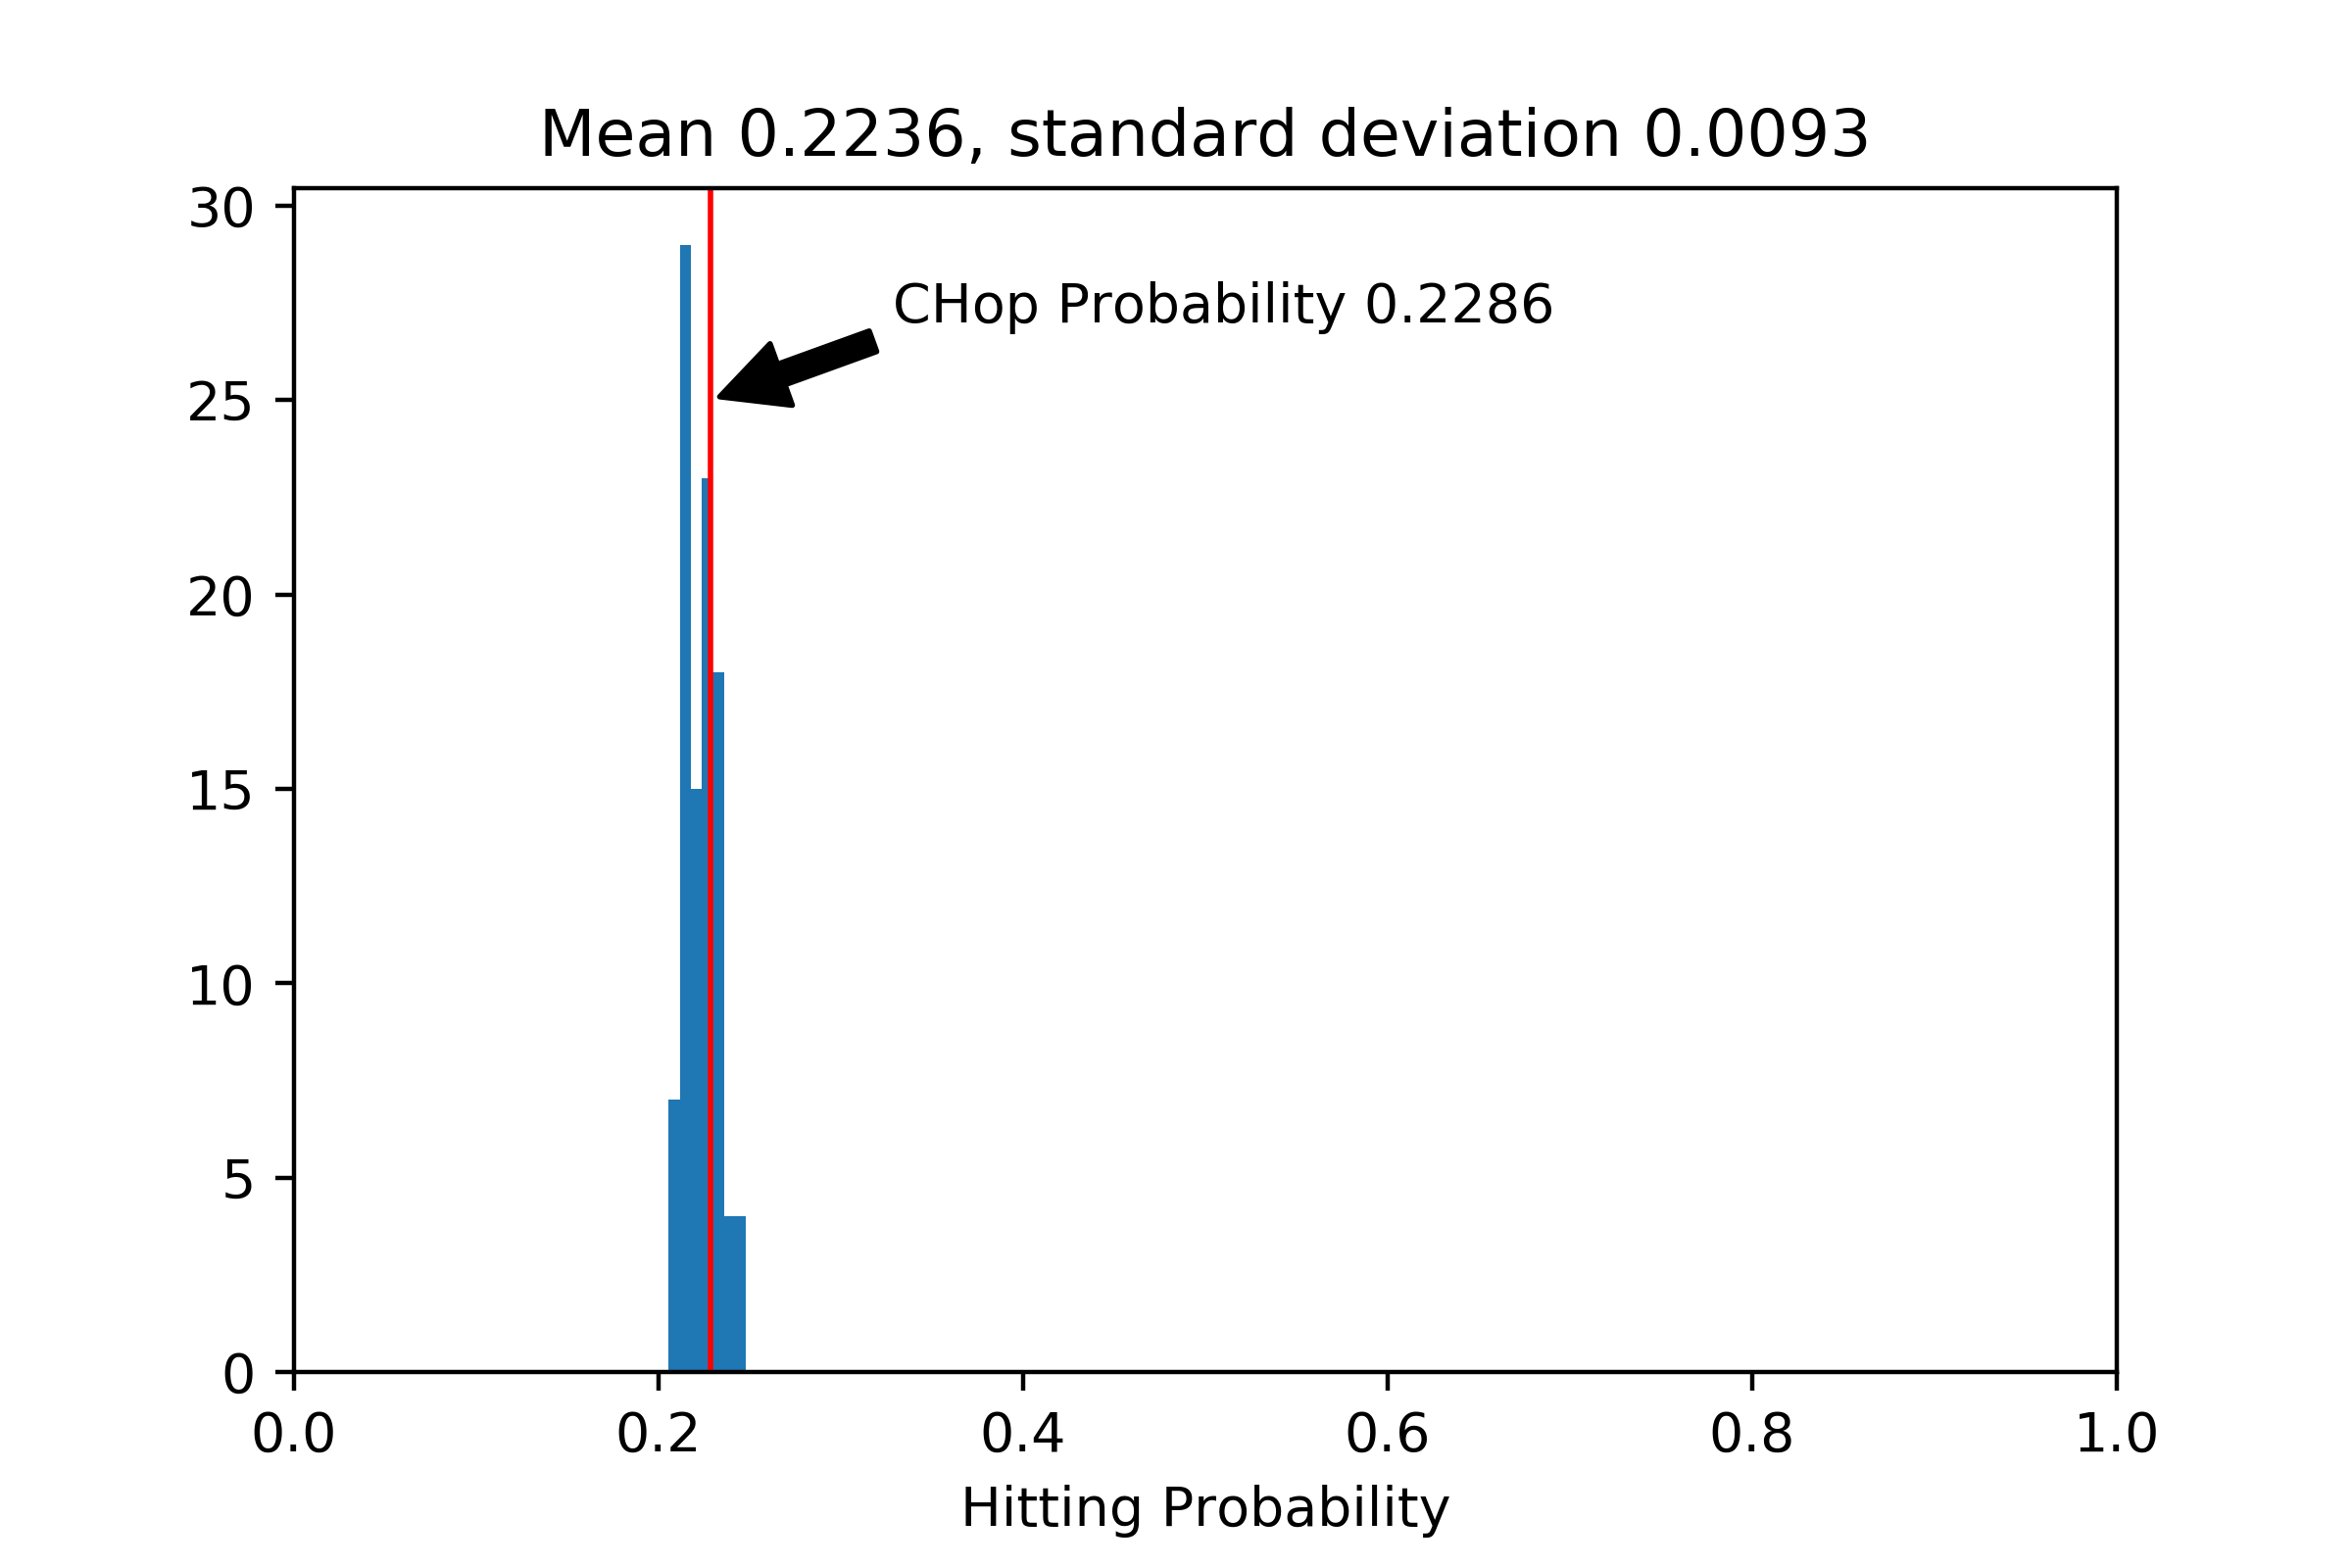
\includegraphics{figs/simple_hitting_prob_hist.png}
\end{figure}


\subsubsection{Capacity Estimation on Flat Energy Landscape}

The second sanity check tests the capacity estimation algorithm employed by CHop. When the energy is flat, we can get an analytical formula for the capacity in the case of concentric spheres. For this test, we try to estimate the capacity $cap(A, \tilde{A})$, with $A=\bb{0, r_A}$ and $\tilde{A}=\bb{0, r_{\tilde{A}}}$, and $U(x)=0,\forall x \in \bb{0, r_{\tilde{A}}} \setminus \bb{0, r_A}$. In this case, the capacity is given analytically as

\begin{equation}
cap(A, \tilde{A}) = \frac{2\pi^{\frac{d}{2}}}{\Gamma(\frac{d}{2})}\frac{d - 2}{r_A^{2 - d} - r_{\tilde{A}}^{2 - d}}
\end{equation}




Take $r_A = 0.1, r_{\tilde{A}} = 0.4$, and $d_A = 0.2$. We can then compare the exact capacity for this case with the capacity given by our capacity estimation algorithm:

\begin{description}
\item[Exact value]  $ 0.080210 $. This is the capacity given by the analytical formula.
\item[Estimate from capacity estimation algorithm]  $ 0.078846 $. To obtain this value we use the version of the capacity estimation algorithm described in the previous section, with parameter values given by 
\begin{equation*}
m = 2, n = 4, 
N_p = 100, N_b = 3,
N_s = 1000
\end{equation*}
We used a 1e-06 time step.
\end{description}


\subsection{Results on Nontrivial Energy Landscape}

In this section, we present some results for the toy model with nontrivial energy landscape around the targets. In addition to testing $\varepsilon$-flatness and CHop probabilities, as we did in previous sanity checks, we further test the efficiency of our capacity estimation algorithm, to demonstrate that our algorithm can accurately estimate the global hitting probabilities while maintaining great advantage over the direct simulations in terms of speed.




We experimented with the toy model with $d = 5$ and
\begin{equation*}
x_A = \begin{pmatrix}%
0.5&0.6&0.0&0.0&0.0%
\end{pmatrix},
r_A = 0.02,
d_A = 0.05,
r_{\tilde{A}} = 0.1
\end{equation*}
for target $A$, and
\begin{equation*}
x_B = \begin{pmatrix}%
-0.7&0.0&0.0&0.0&0.0%
\end{pmatrix},
r_B = 0.04,
d_B = 0.075,
r_{\tilde{B}} = 0.15
\end{equation*}
for target $B$.  We refer the reader to appendix \ref{sec:energy_function} for details on the energy function, as well as the actual parameters we used in our experiments.


\subsubsection{$\varepsilon$-flatness and CHop Probabilities}

We again start by testing the basic idea of CHop: we test our assumption of $\varepsilon$-flatness using direct simulations, to see the applicability of this condition when there is a nontrivial energy landscape. We further compare the CHop Probabilities with the hitting probabilities given by the direct simulations.





\begin{description}
\item[Hitting probabilities estimated with direct simulations:] $\approx 0.8180$.  We run 2000 diffusion simulations at each one of the 100 randomly picked initial locations from $\mathcal{B}(0, 1) \setminus (\tilde{A} \cup \tilde{B})$. For each initial location we obtain an estimate of the hitting probability. The mean of these estimates is 0.8180, standard deviation 0.0096. We used time step of size 1e-05. A histogram of the different hitting probabilities, as well as the CHop probability, is shown in Fig. \ref{fig:nontrivial_hitting_prob_test}. The hitting probabilities from different initial locations are in $[0.7980, 0.8450]$, and the $\varepsilon$-flatness condtion holds with $\varepsilon = 0.0470$.

\item[CHop probability]  0.8274, which is in good agreement with the hitting probabilities we obtained from direct simulations. For the region around $x_A$, we used
\begin{equation*}
m = 2, n = 4, 
N_p = 5000, N_b = 10,
N_s = 2000
\end{equation*}
For the region around $x_B$, we used
\begin{equation*}
m = 2, n = 5, 
N_p = 5000, N_b = 10,
N_s = 2000
\end{equation*}
For estimating both of these capacities, we used a 1e-07 time step.
\end{description}

\begin{figure}
	\caption{\label{fig:nontrivial_hitting_prob_test} We picked 100 random locations for $ X_0 \not\in \mathcal{B}(0, 1) \setminus (\tilde{A} \cup \tilde{B})$. For each location we used 2000 simulations to estimate the probability of hitting $A$ before $B$. The histogram of the 100 estimates is shown below. The $\varepsilon$-flatness condtion holds with $\varepsilon = 0.0470,$ and the CHop probability gives good approximation to this narrow range of hitting probabilities.}
	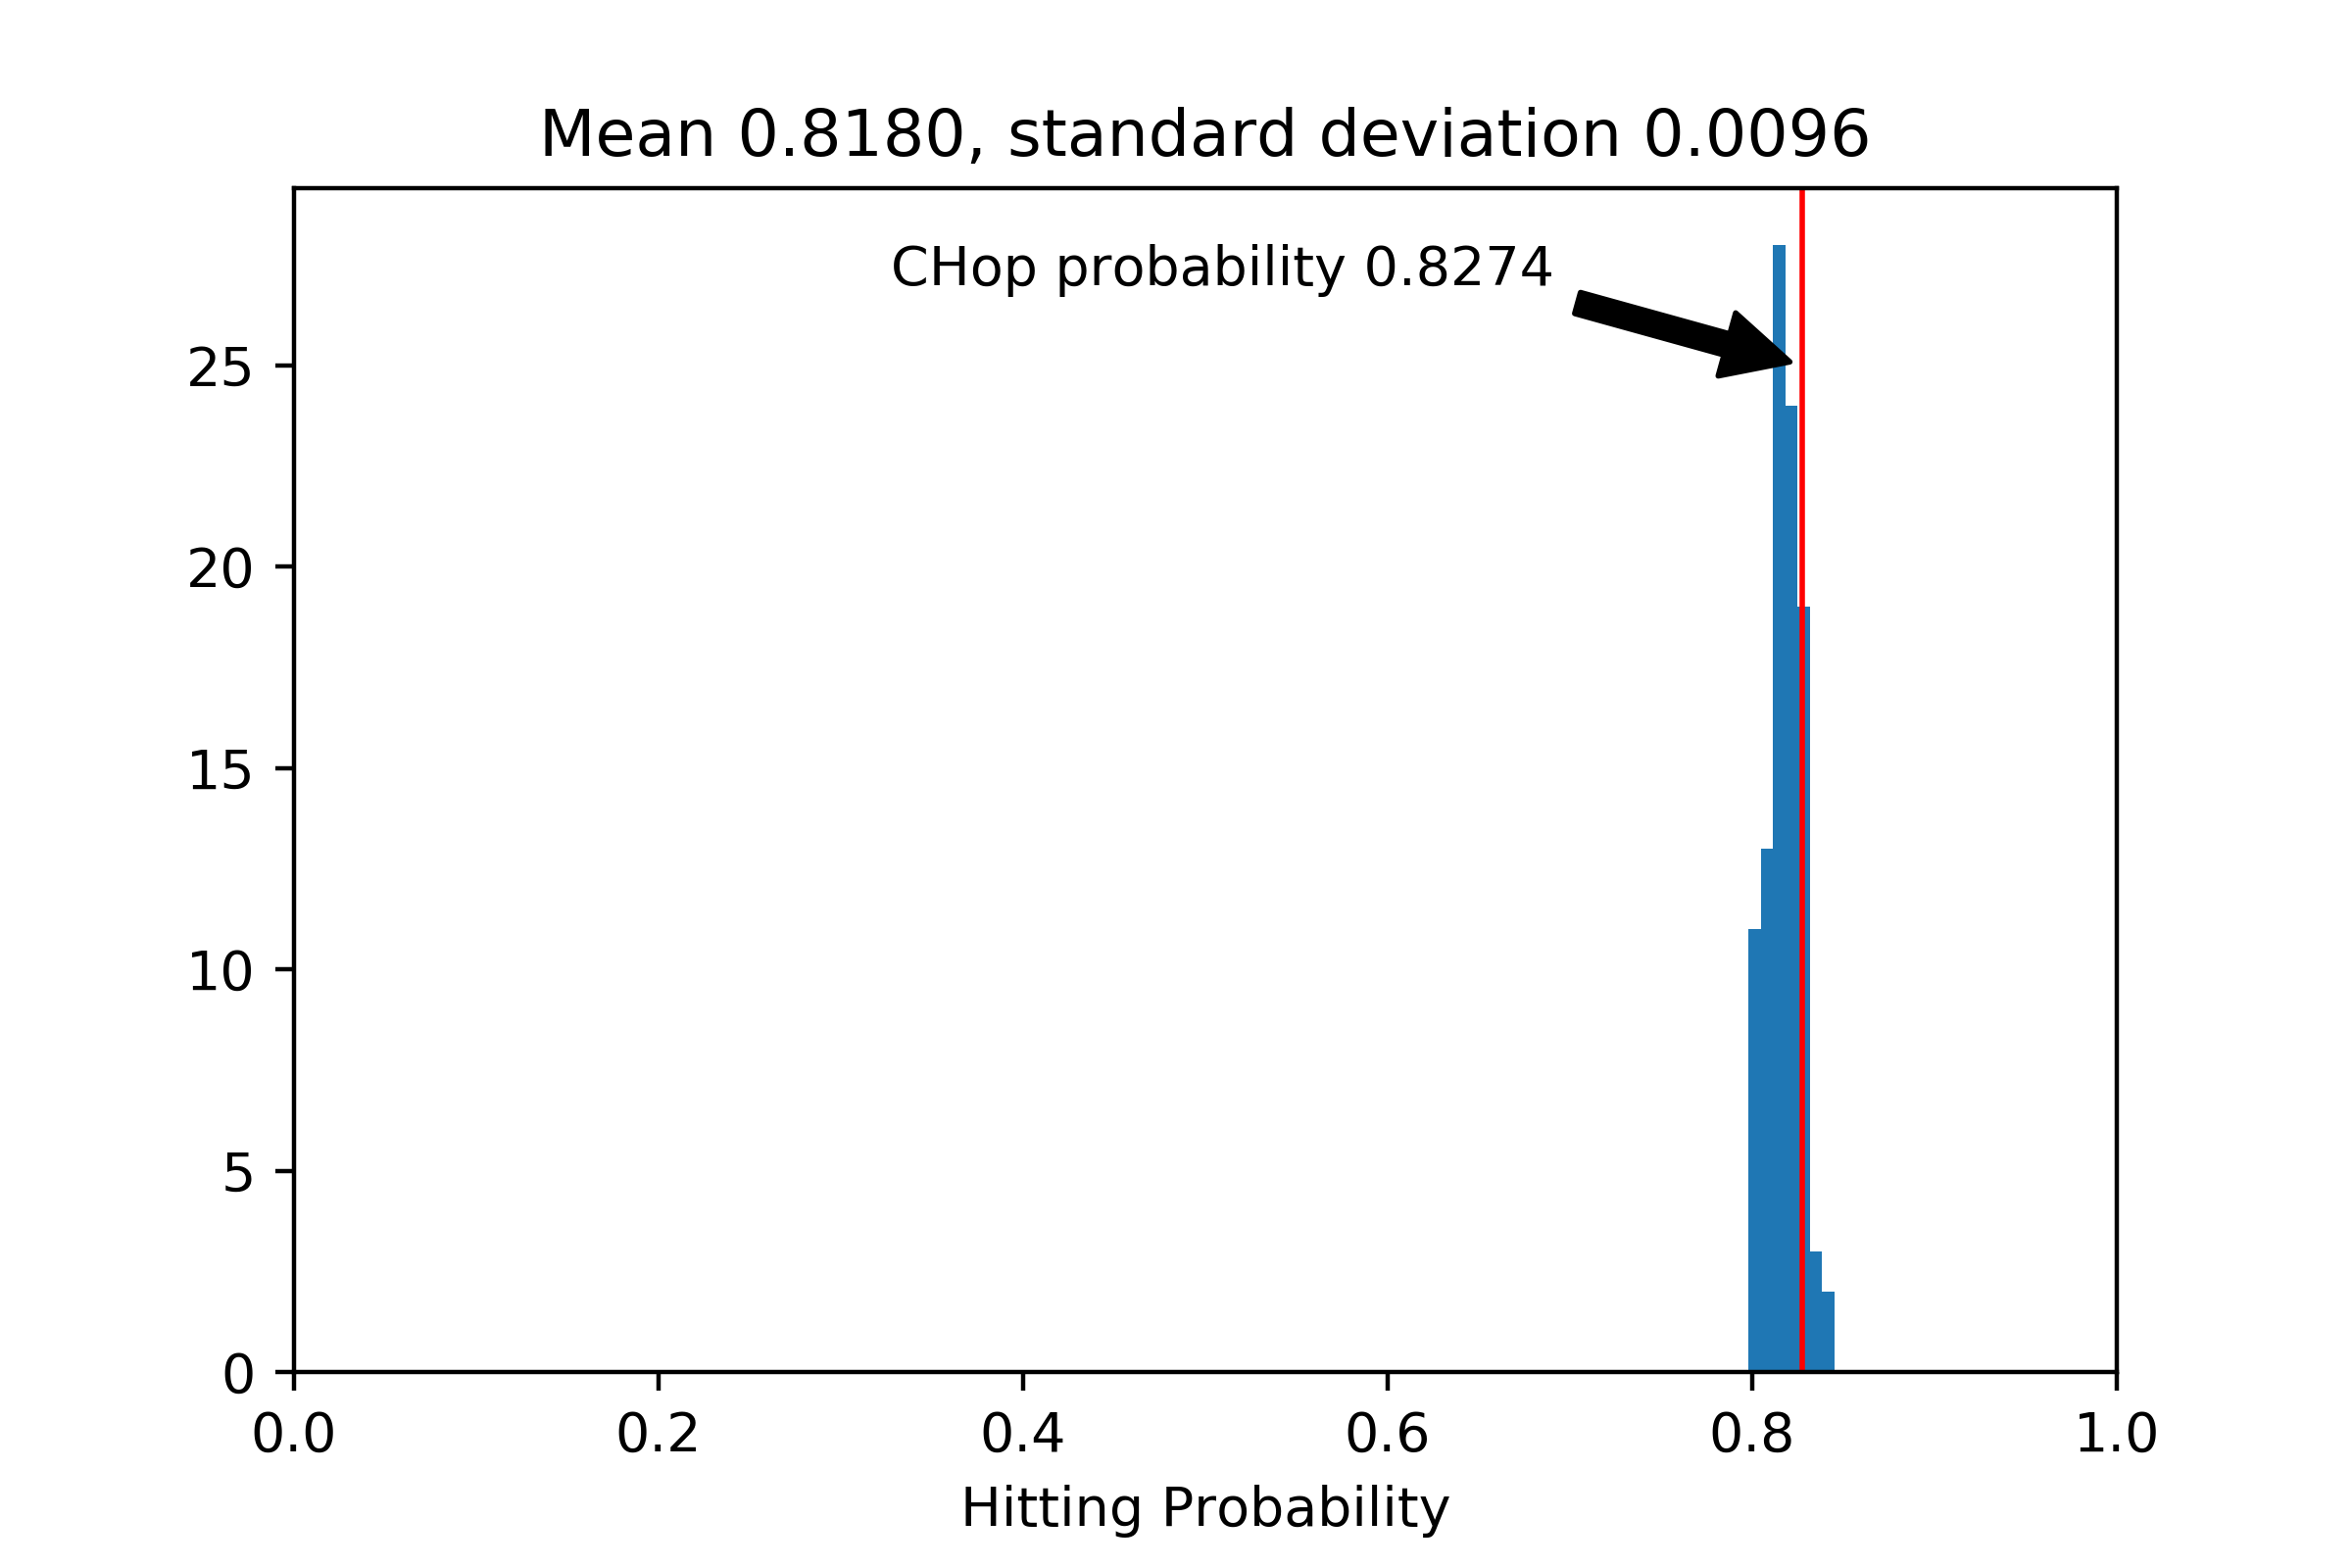
\includegraphics{figs/nontrivial_hitting_prob_hist.png}
\end{figure}


\subsubsection{Efficiency of the Capacity Estimation Algorithm}

To test the efficiency of the algorithm, we compared the time it takes to estimate the hitting probabilities using direct simulations with the time our capacity estimation algorithm needs to estimate the capacities for all targets. Note that in order to make the direct simulations feasible for the $5$-dimensional toy model we are working on, we made our best effort to make the direct simulation fast, including spherical acceleration in the flat region, JIT compilation to remove loop overhead, 24-CPU parallization, and a relatively coarse time step.




\begin{description}
\item[Direct simulation] 89177.87 seconds (3715.74 seconds on 24 CPUs).  This quantity is an average over the amount of time it took to run 2000 simulations for each of the 100 different initial locations, using a relatively coarse time step of 1e-05.  We confirmed that there was no significant overhead due to the parallelization.




\item[CHop speed] 1055.55 seconds on a single CPU. Note that to get an accurate estimate, we need to employ a shorter time step of 1e-07. But this doesn't constitute any computational burden because of the accelerations achieved by CHop.

\end{description}

This reflects an 85-fold acceleration.  Furthermore note that the time-consuming elements of the capacity estimation algorithm are ``embarassingly parallelizable" and should be easy to further accelerate using parallelization.  There was no need to do so in this case because we could easily run the CHop code on our laptops.  However, larger scale problems would certainly benefit from this kind of acceleration.  




The times reported above reflect a particular choice of parameters, but we found that the accuracy of the algorithm was fairly robust to choices of $N_p, N_b$ and $N_s$.  For example, we performed another experiment with a 1e-06 time step, parameters of $ m = 2, n = 4, N_p = 3000, N_b = 5, N_s = 1000 $ for estimating the $A$ capacity, and parameters of $ m = 2, n = 5, N_p = 3000, N_b = 5, N_s = 1000 $ for estimating the $B$ capacity.  The result was an estimate of $0.8420$. This still agrees well with the direct simulations (indeed, there were some initial conditions for which the direct simulation hitting probability estimates agreed with this quantity almost exactly).  Using these parameters, total computation time was reduced to 119.35 seconds, reflecting a 750-fold acceleration.



\section{Conclusions and Future Directions}\label{sec:conclusion}

Using a golf-course energy landscape with multiple targets as a prototypical example, this paper gives new theoretical insights into the commonly encountered entropic barriers in molecular dynamics simulations, from the perspective of hitting probabilities of the targets. A new concept called $\varepsilon$-flatness is proposed to capture the idea of the hitting probabilities being approximately a constant in a set, and $\varepsilon$-flatness is established for a characteristic entropic barrier, our toy model. Further connections are made between the global hitting probabilities of the entropic barriers and the capacities of local sets around the targets, to facilitate the easy understanding of entropic barriers. Inspired by these theoretical developments, we propose CHop as a general and practical method for overcoming entropic barriers, together with an efficient algorithm to deal with the central computational issue of CHop, namely the estimation of capacities.

Extensive numerical results demonstrate that CHop is highly effective in the presence of entropic barriers, both in terms of accuracy and speed, yet future work remains. We see three directions as the most important in further developing the ideas set forth in this paper:
\begin{enumerate}
	\item Move beyond the toy problem in this paper, and make CHop generally applicable to more realistic biomolecular systems. This involves identifying entropic barriers and establishing their $\varepsilon$-flatness in a more general setting, and thinking carefully about the geometry of more realistic biomolecular systems to estimate the capacities of the sets around the targets. Some preliminary discussions are given in this paper, but more work is needed in order to get a clear understanding.
	\item Get results concerning hitting times, in addition to the hitting probabilities talked about in the paper, so that we can fully recover the kinetic information of the system.
	\item Think more about ways to model the configuration space as a hierarchical, nested golf-course, with each target as a mini golf-course inside a larger one, and apply CHop recursively so as to develop a complete model for biomolecular systems, much like kinetic transition networks\cite{Noe2006-cs, Wales2006-ur} and Markov State Models \cite{Pande2010-yi, Chodera2014-bh, Husic2018-xp}
\end{enumerate}

\appendix

\section{Stationary Reversible Diffusion Processes}\label{sec:reversible_diffusion}

In this section, we are going to make formal definitions of stationary
reversible SDEs, and derive some properties that are central to the paper.
Assume $\{X_t\}_{t \geqslant 0}$ is a stationary diffusion process in
$\mathbbm{R}^d$ with invariant measure ${\mu}$. Define $\tau_S
=\ensuremath{\operatorname{int}} \{ t \geqslant 0 : X_t \in S \} , \text{ for
} S \subset \mathbbm{R}^d$. We first define the notion of reversibility for
general diffusion processes. Our discussion here follows Section 4.6 of
Pavliotis\cite{Pavliotis2016-xn}.

\begin{definition}
(Definition 4.3 of Pavliotis\cite{Pavliotis2016-xn}) A stationary stochastic
process $\{X_t\}_{t \geqslant 0}$ is time-reversible if its law is invariant under time
reversal: for every $T \in (0, + \infty)$, $\{X_t\}_{t \geqslant 0}$ and the time-reversed
process $\{X_{T - t}\}_{t \geqslant 0}$ have the same distribution.
\end{definition}

Recall that a diffusion pross can be characterized by its generator. It turns
out the reversibility of a stationary diffusion process can also be
characterized by its generator. We have

\begin{theorem}
\label{thm:reversibility}(Theorem 4.5 of Pavliotis\cite{Pavliotis2016-xn}) A
stationary diffusion process $\{X_t\}_{t \geqslant 0}$ in $\mathbbm{R}^d$ with generator
$\mathcal{L}$ and invariant measure ${\mu}$ is reversible if and only if
its generator is self-adjoint in $L^2 (\mathbbm{R}^d ; {\mu})$.
\end{theorem}

For the rest of this section, we turn to the case where the stationary
diffusion process $\{X_t\}_{t \geqslant 0}$ satisfies the SDE
\[ \mathrm{d} X_t = b (X_t) \mathrm{d} t + \sigma (X_t) \mathrm{d} W_t \]
where $b (\cdot) : \mathbbm{R}^d \rightarrow \mathbbm{R}^d$ and $\sigma
(\cdot) : \mathbbm{R}^d \rightarrow \mathbbm{R}^{d \times m}$ are
differentiable vector-valued and matrix-valued functions. Define $a (x) =
\sigma (x) \sigma (x)^T$. We assume the invariant measure may be written as
${\mu}= e^{- U (x)}$, where $U (x)$ is a scalar function and can be
thought of as a generalized potential.

Recall that, for this SDE, the generator $\mathcal{L}$ is given by
\[ (\mathcal{L} f) (x) = b (x) \cdot \nabla f (x) + \frac{1}{2} a (x) :
\nabla^2 f (x) \]
where $\cdot$ represents the inner product, $:$ represents the Frobenius inner
product, and $\nabla^2 f (x)$ represents the Hessian matrix of the function $f
(x)$, i.e.
\[ (\mathcal{L} f) (x) = \sum_{i = 1}^d b_i (x) \frac{\partial f
(x)}{\partial x_i} + \frac{1}{2} \sum_{i = 1}^d \sum_{j = 1}^d a_{ij} (x)
\frac{\partial^2 f (x)}{\partial x_i \partial x_j} \]
Using $m$ to denote the Lebesgue measure, the adjoint of $\mathcal{L}$ in $L^2
(\mathbbm{R}^d ; m)$ is the Fokker Planck operator
\[ (\mathcal{L}^{\ast} f) (x) = - \nabla \cdot (b (x) f (x)) + \frac{1}{2}
\nabla^2 : (a (x) f (x)) = - \sum_{i = 1}^d \frac{\partial (b_i (x) f
(x))}{\partial x_i} + \frac{1}{2} \sum_{i = 1}^d \sum_{j = 1}^d
\frac{\partial^2 (a_{ij} (x) f (x))}{\partial x_i \partial x_j} \]
Note that we can further write the Fokker Planck operator $\mathcal{L}^{\ast}$
as $\mathcal{L}^{\ast} = \nabla \cdot J$, where
\[ (J f) (x) = - b (x) f (x) + \frac{1}{2} \nabla \cdot (a (x) f (x)) \]
i.e.
\[ (J f)_i (x) = - b_i (x) f (x) + \frac{1}{2} \sum_{j = 1}^d \frac{\partial
(a_{ij} (x) f (x))}{\partial x_j} \]
In the case where $f (x)$ is a density function, $(J f) (x)$ gives us the
probability flux of the Markov process starting at the distribution $f (x)$.

Combining these basic formulas with Theorem \ref{thm:reversibility}, it's easy
to see that the condition for the SDE being reversible is
\[ (\mathcal{L}^{\ast} f e^{-U}) (x) = e^{- U (x)} (\mathcal{L} f) (x),
\forall f \]
Alternatively, we have the following proposition

\begin{proposition}
(Proposition 4.5 of Pavliotis\cite{Pavliotis2016-xn}) $X_t$ is reversible if
and only if $(J e^{- U })(x)$ holds, or equivalently, $b (x) = \frac{1}{2}
\nabla \cdot a (x) - \frac{1}{2} a (x) \nabla U (x)$.
\end{proposition}

We establish a useful property of stationary reversible SDEs.

\begin{proposition}\label{prop:property_reversible_sde}
If $X_t$ is reversible, then $(J f e^{- U })(x) = \frac{1}{2} e^{- U
(x)} a (x) \nabla f (x) , \forall f$.
\end{proposition}

\noindent\textbf{Proof\ }This result can be established by using the
definition of $J$, the property $(J e^{- U })(x) = 0$, and straightforward
calculations. We have
\begin{eqnarray*}
(J f e^{- U })(x) & = & - b (x) f (x) e^{- U (x)} + \frac{1}{2} \nabla
\cdot (a (x) f (x) e^{- U (x)})\\
\nabla \cdot (a (x) f (x) e^{- U (x)}) & = & f (x) \nabla \cdot (a (x) e^{-
U (x)}) + e^{- U (x)} a (x) \nabla f (x)\\
\Longrightarrow (J f e^{- U })(x) & = & f (x) \left[ - b (x) e^{- U (x)}
+ \frac{1}{2} \nabla \cdot (a (x) e^{- U (x)}) \right] + \frac{1}{2} e^{- U
(x)} a (x) \nabla f (x)\\
& = & f (x) (J e^{- U })(x) + \frac{1}{2} e^{- U (x)} a (x) \nabla f (x)\\
& = & \frac{1}{2} e^{- U (x)} a (x) \nabla f (x)
\end{eqnarray*}\hspace*{\fill}$\Box$\medskip

We next move on to the definition of Dirichlet form and capacity for
stationary reversible SDEs. We have the following definitions

\begin{definition}
Assume $X_t$ is a stationary reversible SDE with invariant measure
${\mu}= e^{- U (x)} \mathrm{d} x$, the Dirichlet form of $X_t$ is given
by
\[ \mathcal{E} (f, g) = \frac{1}{2} \int_{\mathbbm{R}^d} \nabla f (x)^T a
(x) \nabla g (x) e^{- U (x)} \mathrm{d} x \]
\end{definition}

Note that in the case of an SDE in $\Omega$ with reflecting boundaries on
$\partial \Omega$, the stationary measure ${\mu}$ is restricted in
$\Omega$. In this case, the Dirichlet form is given by
\[ \mathcal{E} (f, g) = \frac{1}{2} \int_{\Omega} \nabla f (x)^T a (x) \nabla
g (x) e^{- U (x)} \mathrm{d} x \]
So this definition also applies to SDEs with reflecting boundaries, which is
the main object of interest in this paper. In what follows, w.l.o.g., we are
going to use $\Omega$ to denote the state space of the process.

\begin{definition}
Let $A \subset \tilde{A} \subset \Omega$ be non-empty. Assume we have an
open set $D \subset \Omega$ for which $\partial D = \partial A \cup \partial
\tilde{A}$ and is regular (in the sense of Theorem 7.17 in
Bovier\cite{Bovier2016-ez}). Denote the Dirichlet form of the reversible
stationary diffusion process $X_t$ in $\Omega$ with invariant measure
${\mu}= e^{- U (x)} \mathrm{d} x$ by $\mathcal{E}$. Let $\mathcal{H}_{A,
\tilde{A}}$ be the space of functions $f$ such that
\begin{enumerate}
\item $f \in H^1$, where $H^1$ is the Soblev space of weakly
differentiable functions

\item $\mathcal{E} (f, f) < \infty$

\item $f \geqslant 1$ on $\partial A$ and $f \leqslant 0$ on $\partial
\tilde{A}$
\end{enumerate}
The capacity $\ensuremath{\operatorname{cap}} (A, \tilde{A})$ is defined as
\[ \ensuremath{\operatorname{cap}} (A, \tilde{A}) = \inf_{f \in
\mathcal{H_{A, \tilde{A}}}} \mathcal{E} (f, f) \]
\end{definition}

Before we state the basic properties of the capacity
$\ensuremath{\operatorname{cap}} (\tilde{A}, \tilde{A})$, we are also going to
define the Dirichlet problem. This problem turns out to be just another
perspective on the same minimization problem which appears in the definition
of the capacity.

\begin{definition}
Let $A, B \subset \Omega$ be non-empty and disjoint. Assume we have an open
set $D \subset \Omega$ for which $\partial D = \partial A \cup \partial B$
and is regular. Given a stationary diffusion process $X_t$ in $\Omega$ with
generator $\mathcal{L}$, the Dirichlet problem is defined as the partial
differential equation
\[ - (\mathcal{L} h) (x) = 0, \forall x \in D \]
with boundary conditions
\begin{eqnarray*}
h (x) & = & 1, x \in A\\
h (x) & = & 0, x \in B
\end{eqnarray*}
\end{definition}

Under certain regularity conditions (in the form of Theorem 7.17 in
Bovier\cite{Bovier2016-ez}), the solution $h_{A, B} (x)$ exists and is
unique, and has the probabilistic interpretation that
\[ h_{A, B} (x) =\mathbbm{P} (X_{\tau_{A \cup B}} \in A|X_0 = x) \]
i.e. $h_{A, B} (x)$ is the probability for $X_t$ to hit $A$ first before
hitting $B$ if we start the process at $x$. This is the celebrated
{\itshape{Dirichlet Principle}}.

Armed with this definition, we are ready to state some basic properties of the
capacity.

\begin{proposition}\label{prop:capacity}
The capacity $\ensuremath{\operatorname{cap}} (A, \tilde{A})$ satisfies the
following properties
\begin{enumerate}
\item (Probabilistic interpretation) If $\mathcal{H}_{A, \tilde{A}} \neq
\varnothing$, then the infimum in the definition of
$\ensuremath{\operatorname{cap}} (A, \tilde{A})$ is attained uniquely at
the solution to the corresponding Dirichlet problem $h_{A, \tilde{A}^c}$,
i.e. $\ensuremath{\operatorname{cap}} (A, \tilde{A}) = \mathcal{E} (h_{A,
\tilde{A}^c}, h_{A, \tilde{A}^c})$.

\item (Additivity) The capacity is additive, i.e. if we have $A \subset
\tilde{A} \subset \Omega$ and $B \subset \tilde{B} \subset \Omega$ where
$\tilde{A}$ and $\tilde{B}$ are disjoint, then we have
\[ \ensuremath{\operatorname{cap}} (A \cup B, \tilde{A} \cup \tilde{B})
=\ensuremath{\operatorname{cap}} (A, \tilde{A})
+\ensuremath{\operatorname{cap}} (B, \tilde{B}) \]
\end{enumerate}
\end{proposition}

\noindent\textbf{Proof\ }
\begin{enumerate}
\item Refer to Theorem 7.33 of Bovier\cite{Bovier2016-ez}

\item By definition, we have
\begin{eqnarray*}
h_{A, \widetilde{A^{}}^c} (x) & = & 0, \forall x \in \tilde{A}^c\\
h_{B, \tilde{B}^c} (x) & = & 0, \forall x \in \tilde{B}^c
\end{eqnarray*}
which implies
\begin{eqnarray*}
\nabla h_{A, \widetilde{A^{}}^c} (x) & = & 0, \forall x \in \tilde{A}^c\\
\nabla h_{B, \tilde{B}^c} (x) & = & 0, \forall x \in \tilde{B}^c
\end{eqnarray*}
Since $\tilde{A}$ and $\tilde{B}$ are disjoint, using the probabilistic interpretation, it's easy to see that
\begin{eqnarray*}
h_{A \cup B, (\tilde{A} \cup \tilde{B})^c} (x) & = & h_{A,
\widetilde{A^{}}^c} (x), \forall x \in \tilde{A}\\
h_{A \cup B, (\tilde{A} \cup \tilde{B})^c} (x) & = & h_{B, \tilde{B}^c}
(x), \forall x \in \tilde{B}
\end{eqnarray*}
Furthermore, we have $h_{A \cup B, (\tilde{A} \cup \tilde{B})^c} (x) = 0, \forall x \in (\tilde{A} \cup \tilde{B})^c$, which implies
\[ \nabla h_{A \cup B, (\tilde{A} \cup \tilde{B})^c} (x) = 0, \forall x \in
(\tilde{A} \cup \tilde{B})^c \]
Since $X_t$ is reversible, using 1, we have
\begin{eqnarray*}
&  & \tmop{cap} (A \cup B, \tilde{A} \cup \tilde{B})\\
& = & \mathcal{E} (h_{A \cup B, (\tilde{A} \cup \tilde{B})^c}, h_{A \cup
B, (\tilde{A} \cup \tilde{B})^c})\\
& = & \frac{1}{2} \int_{\Omega} (\nabla h_{A \cup B, (\tilde{A}
\cup \tilde{B})^c} (x))^T a (x) \nabla h_{A \cup B, (\tilde{A} \cup
\tilde{B})^c} (x) e^{- U (x)} \mathd x\\
& = & \frac{1}{2} \int_{\tilde{A}} (\nabla h_{A \cup B, (\tilde{A} \cup
\tilde{B})^c} (x))^T a (x) \nabla h_{A \cup B, (\tilde{A} \cup
\tilde{B})^c} (x) e^{- U (x)} \mathd x\\
& + & \frac{1}{2} \int_{\tilde{B}} (\nabla h_{A \cup B, (\tilde{A} \cup
\tilde{B})^c} (x))^T a (x) \nabla h_{A \cup B, (\tilde{A} \cup
\tilde{B})^c} (x) e^{- U (x)} \mathd x\\
& + & \frac{1}{2} \int_{(\tilde{A} \cup \tilde{B})^c} (\nabla h_{A \cup
B, (\tilde{A} \cup \tilde{B})^c} (x))^T a (x) \nabla h_{A \cup B,
(\tilde{A} \cup \tilde{B})^c} (x) e^{- U (x)} \mathd x\\
& = & \frac{1}{2} \int_{\tilde{A}} \left( \nabla h_{A,
\widetilde{A^{}}^c} (x) \right)^T a (x) \nabla h_{A, \widetilde{A^{}}^c}
(x) (x) e^{- U (x)} \mathd x\\
& + & \frac{1}{2} \int_{\tilde{B}} (\nabla h_{B, \tilde{B}^c} (x))^T a
(x) \nabla h_{B, \tilde{B}^c} (x) (x) e^{- U (x)} \mathd x\\
& = & \frac{1}{2} \int_{\Omega} \left( \nabla h_{A,
\widetilde{A^{}}^c} (x) \right)^T a (x) \nabla h_{A, \widetilde{A^{}}^c}
(x) (x) e^{- U (x)} \mathd x\\
& + & \frac{1}{2} \int_{\Omega} (\nabla h_{B, \tilde{B}^c} (x))^T
a (x) \nabla h_{B, \tilde{B}^c} (x) (x) e^{- U (x)} \mathd x\\
& = & \mathcal{E} \left( h_{A, \widetilde{A^{}}^c} (x), h_{A,
\widetilde{A^{}}^c} (x) \right) + \mathcal{E} (h_{B, \tilde{B}^c} (x),
h_{B, \tilde{B}^c} (x))\\
& = & \tmop{cap} (A, \tilde{A}) + \tmop{cap} (B, \tilde{B})
\end{eqnarray*}
which proves the result.
\end{enumerate}
\hspace*{\fill}$\Box$\medskip

\section{Proof of the Main Theorem}\label{sec:proof_thm}

\noindent\textbf{Proof of Theorem \ref{thm:main_thm}\ }
Note that because of the probabilistic interpretation of the capacity, we have
\[ \mathcal{E} (u, u) = \tmop{cap} (A, B^c) = \inf_{f \in \mathcal{H}_{A, B^c}} \mathcal{E} (f, f) \]
Recall that, since $X_t$ is reversible, the Dirichlet form takes the form
\[ \mathcal{E} (f, f) = \frac{1}{2} \int_{\Omega} (\nabla f (x))^T a
(x) \nabla f (x) e^{- F (x)} \mathd x \]
Intuitively, $\forall f \in \mathcal{H}_{A, B^c}$, the Dirichlet form $\mathcal{E} (f, f)$ measures the costs (in terms of suitable norm of the gradient of $f$) we need to pay to grow the function $f$ from being 0 on $\partial B$ to being 1 on $\partial A$. Because of the definition of $u$, $\forall f \in \mathcal{H}_{A, B^c}$, we have the upper bound \[ \mathcal{E} (u, u) \leqslant \mathcal{E} (f, f) \] If we have a relatively tight upper-bound for $\mathcal{E} (u, u)$, it would place significant constraints on the function $u$ itself, because of the $\varepsilon$-flatness of $M$. Since the function $u$ can grow by at most $\varepsilon$ within $M$, most of its growth from being $0$ on $\partial B$ to being 1 on $\partial A$ would have to be done within $\tilde{A} / A$ and $\tilde{B} / B$. Increasing the amount of growth needed within a region by $k$ times would approximately increase the contribution to the Dirichlet form within this region by $k^2$ times, so the value of $u$ within $M$ has to be carefully balanced. Being too far away from 0 would make
\[ \frac{1}{2} \int_{\tilde{B} / B} (\nabla u (x))^T a (x) \nabla u (x) e^{- U (x)} \mathd x \]
explode, while being too far away from 1 would make
\[ \frac{1}{2} \int_{\tilde{A} / A} (\nabla u (x))^T a (x) \nabla u (x) e^{- U (x)} \mathd x \]
explode. Both cases would violate the upper bound we have already established for $\mathcal{E} (u, u)$.

Formally, we first establish the upper bound by making use of $h_{A,
\tilde{A}^c}$ and $h_{B, \widetilde{B}^c}$. $\forall c \in (0, 1)$, define
\[ \hat{u}_c (x) = \left\{ \begin{array}{l}
c, \tmop{if} x \in M\\
(1 - c) h_{A, \widetilde{A}^c} (x) + c, \tmop{if} x \in \tilde{A}\\
c (1 - h_{B, \widetilde{B}^c} (x)), \tmop{if} x \in \tilde{B}
\end{array} \right. \]
Obviously $\hat{u}_c \in \mathcal{H_{}}_{A, B^c}$, which implies
\begin{eqnarray*}
&  & \mathcal{E} (u, u)\\
& \leqslant & \mathcal{E} (\hat{u}_c, \hat{u}_c)\\
& = & \frac{1}{2} \int_{\Omega} (\nabla \hat{u}_c (x))^T a (x)
\nabla \hat{u}_c (x) e^{- U (x)} \mathd x\\
& = & \frac{1}{2} \int_{\tilde{A}} (\nabla \hat{u}_c (x))^T a (x) \nabla
\hat{u}_c (x) e^{- U (x)} \mathd x + \frac{1}{2} \int_{\tilde{B}} (\nabla
\hat{u}_c (x))^T a (x) \nabla \hat{u}_c (x) e^{- U (x)} \mathd x\\
& = & \frac{1}{2} (1 - c)^2 \int_{\tilde{A}} (\nabla h_{A, \widetilde{A}^c}
(x))^T a (x) \nabla h_{A, \widetilde{A}^c} (x) e^{- U (x)} \mathd x\\
& + & \frac{1}{2} c^2 \int_{\tilde{B}} (\nabla h_{B, \widetilde{B}^c}
(x))^T a (x) \nabla h_{B, \widetilde{B}^c} (x) e^{- U (x)} \mathd x\\
& = & (1 - c)^2 \tmop{cap} (A, \tilde{A}) + c^2 \tmop{cap} (B, \tilde{B}),
\forall c \in (0, 1)
\end{eqnarray*}
Minimizing this w.r.t. $c$, we get an upper bound for $\mathcal{E} (u, u)$:
\[ \mathcal{E} (u, u) \leqslant \frac{\tmop{cap} (A, \tilde{A}) \tmop{cap} (B,
\tilde{B})}{\tmop{cap} (A, \tilde{A}) + \tmop{cap} (B, \tilde{B})} \]
Next, note that, because $M$ is an $\varepsilon$-flat barrier for $u$, we have
\[ \sup_{x \in M} u (x) - \inf_{x \in M} u (x) < \varepsilon \]
Define $m = \frac{1}{2} (\sup_{x \in M} u (x) + \inf_{x \in M} (u (x)))$, we have
\begin{equation}
\label{epsilonflat}
| u (x) - m | < \frac{\varepsilon}{2}, \forall x \in M 
\end{equation}
And we have $u (x) \geqslant m - \frac{\varepsilon}{2}, \forall x \in \partial \tilde{B}$, and $u (x) \leqslant m + \frac{\varepsilon}{2}, \forall x \in \partial \tilde{A}$. Since $u (x) = 1, \forall x \in A$, and $u (x) = 0, \forall x \in B$, define
\begin{eqnarray*}
u_A (x) & = & \left\{ \begin{array}{l}
\frac{u (x) - m - \frac{\varepsilon}{2}}{1 - m - \frac{\varepsilon}{2}}, x
\in \tilde{A}\\
0, x \nin \tilde{A}
\end{array} \right., \tmop{if} m + \frac{\varepsilon}{2} < 1\\
u_B (x) & = & \left\{ \begin{array}{l}
1 - \frac{1}{m - \frac{\varepsilon}{2}} u (x), x \in \tilde{B}\\
0, x \nin \tilde{B}
\end{array} \right., \tmop{if} m > \frac{\varepsilon}{2}
\end{eqnarray*}
we have $u_A \in \mathcal{H}_{A, \tilde{A}}, u_B \in \mathcal{H}_{B,
\tilde{B}}$, and
\begin{eqnarray*}
&  & \mathcal{E} (u, u)\\
& = & \frac{1}{2} \int_{\Omega} (\nabla u (x))^T a (x) \nabla u (x)
e^{- U (x)} \mathd x\\
& \geqslant & \frac{1}{2} \int_{\tilde{A}} (\nabla u (x))^T a (x) \nabla u
(x) e^{- U (x)} \mathd x + \frac{1}{2} \int_{\tilde{B}} (\nabla u (x))^T a
(x) \nabla u (x) e^{- U (x)} \mathd x\\
& \geqslant & \left( 1 - m - \frac{\varepsilon}{2} \right)^2 \mathcal{E}
(u_A, u_A) \chi_{\left( 0, 1 - \frac{\varepsilon}{2} \right)} (m) + \left( m
- \frac{\varepsilon}{2} \right)^2 \mathcal{E} (u_B, u_B) \chi_{\left(
\frac{\varepsilon}{2}, 1 \right)} (m)\\
& \geqslant & \left( 1 - m - \frac{\varepsilon}{2} \right)^2 \tmop{cap} (A,
\tilde{A}) \chi_{\left( 0, 1 - \frac{\varepsilon}{2} \right)} (m) + \left( m
- \frac{\varepsilon}{2} \right)^2 \tmop{cap} (B, \tilde{B}) \chi_{\left(
\frac{\varepsilon}{2}, 1 \right)} (m)
\end{eqnarray*}
Combining this with the upper bound we already establish, we have
\[ \left( 1 - m - \frac{\varepsilon}{2} \right)^2 \tmop{cap} (A, \tilde{A})
\chi_{\left( 0, 1 - \frac{\varepsilon}{2} \right)} (m) + \left( m -
\frac{\varepsilon}{2} \right)^2 \tmop{cap} (B, \tilde{B}) \chi_{\left(
\frac{\varepsilon}{2}, 1 \right)} (m) \leqslant \frac{\tmop{cap} (A,
\tilde{A}) \tmop{cap} (B, \tilde{B})}{\tmop{cap} (A, \tilde{A}) +
\tmop{cap} (B, \tilde{B})} \]
In the typical case where $m \in \left( \frac{\varepsilon}{2}, 1 - \frac{\varepsilon}{2} \right)$, the above constraint becomes the quadratic inequality
\[ \left( 1 - m - \frac{\varepsilon}{2} \right)^2 \tmop{cap} (A, \tilde{A}) +
\left( m - \frac{\varepsilon}{2} \right)^2 \tmop{cap} (B, \tilde{B})
\leqslant \frac{\tmop{cap} (A, \tilde{A}) \tmop{cap} (B,
\tilde{B})}{\tmop{cap} (A, \tilde{A}) + \tmop{cap} (B, \tilde{B})} \]
Solving this, we have
\begin{eqnarray*}
m & \geqslant & \frac{\tmop{cap} (A, \tilde{A}) \tmop{cap} (B,
\tilde{B})}{\tmop{cap} (A, \tilde{A}) + \tmop{cap} (B, \tilde{B})} +
\frac{\varepsilon}{2} \frac{\tmop{cap} (B, \tilde{B}) - \tmop{cap} (A,
\tilde{A})}{\tmop{cap} (A, \tilde{A}) + \tmop{cap} (B, \tilde{B})} - \frac{2
\sqrt{\tmop{cap} (A, \tilde{A}) \tmop{cap} (B, \tilde{B})
\frac{\varepsilon}{2} \left( 1 - \frac{\varepsilon}{2} \right)}}{\tmop{cap}
(A, \tilde{A}) + \tmop{cap} (B, \tilde{B})}\\
m & \leqslant & \frac{\tmop{cap} (A, \tilde{A}) \tmop{cap} (B,
\tilde{B})}{\tmop{cap} (A, \tilde{A}) + \tmop{cap} (B, \tilde{B})} +
\frac{\varepsilon}{2} \frac{\tmop{cap} (B, \tilde{B}) - \tmop{cap} (A,
\tilde{A})}{\tmop{cap} (A, \tilde{A}) + \tmop{cap} (B, \tilde{B})} + \frac{2
\sqrt{\tmop{cap} (A, \tilde{A}) \tmop{cap} (B, \tilde{B})
\frac{\varepsilon}{2} \left( 1 - \frac{\varepsilon}{2} \right)}}{\tmop{cap}
(A, \tilde{A}) + \tmop{cap} (B, \tilde{B})}
\end{eqnarray*}
from which we deduce that $\left| m - \frac{\tmop{cap} (A, \tilde{A}) \tmop{cap} (B, \tilde{B})}{\tmop{cap} (A, \tilde{A}) + \tmop{cap} (B, \tilde{B})} \right| \leqslant \frac{\varepsilon}{2} + \sqrt{\frac{\varepsilon}{2}}$.

In the extreme cases where $m$ is outside $\left( \frac{\varepsilon}{2}, 1 - \frac{\varepsilon}{2} \right)$, in order for the inequality to hold, we would need to have $\frac{\tmop{cap} (A, \tilde{A})}{\tmop{cap} (A, \tilde{A}) + \tmop{cap} (B, \tilde{B})}$ to be very small when \ $m \leqslant \frac{\varepsilon}{2}$, and very big when $m \geqslant 1 - \frac{\varepsilon}{2}$, which would give us the desired bound. Because of symmetry, the proofs for these two cases are essentially the same. We take the case $m \leqslant \frac{\varepsilon}{2}$ as an example. In this case, we have the inequality
\[ \left( 1 - m - \frac{\varepsilon}{2} \right)^2 \tmop{cap} (A, \tilde{A})
\leqslant \frac{\tmop{cap} (A, \tilde{A}) \tmop{cap} (B,
\tilde{B})}{\tmop{cap} (A, \tilde{A}) + \tmop{cap} (B, \tilde{B})} \]
which implies
\[ \frac{\tmop{cap} (B, \tilde{B})}{\tmop{cap} (A, \tilde{A}) + \tmop{cap} (B,
\tilde{B})} \geqslant (1 - \varepsilon)^2 \]
from which we have
\begin{eqnarray*}
&  & \frac{\tmop{cap} (A, \tilde{A})}{\tmop{cap} (A, \tilde{A}) +
\tmop{cap} (B, \tilde{B})}\\
& = & 1 - \frac{\tmop{cap} (B, \tilde{B})}{\tmop{cap} (A, \tilde{A}) +
\tmop{cap} (B, \tilde{B})}\\
& \leqslant & 1 - (1 - \varepsilon)^2\\
& = & 2 \varepsilon - \varepsilon^2
\end{eqnarray*}
It's easy to see that when $\varepsilon \leqslant \frac{2}{9}$, we have
\[ 2 \varepsilon - \varepsilon^2 - \left( \frac{\varepsilon}{2} +
\sqrt{\frac{\varepsilon}{2}} \right) = \frac{3 \varepsilon}{2} -
\varepsilon^2 - \sqrt{\frac{\varepsilon}{2}} = \sqrt{\varepsilon} \left(
\frac{3}{2} \sqrt{\varepsilon} - \varepsilon^{\frac{3}{2}} -
\sqrt{\frac{1}{2}} \right) \leqslant \sqrt{\varepsilon} \left( \frac{3}{2}
\frac{\sqrt{2}}{3} - \frac{\sqrt{2}}{2} \right) = 0 \]
As a result, we have both $\frac{\tmop{cap} (A, \tilde{A})}{\tmop{cap} (A, \tilde{A}) + \tmop{cap} (B, \tilde{B})} \leqslant \frac{\varepsilon}{2} + \sqrt{\frac{\varepsilon}{2}}$ and $m \leqslant \frac{\varepsilon}{2} \leqslant \frac{\varepsilon}{2} + \sqrt{\frac{\varepsilon}{2}}$, which implies
\[ \left| m - \frac{\tmop{cap} (A, \tilde{A})}{\tmop{cap} (A, \tilde{A}) +
\tmop{cap} (B, \tilde{B})} \right| \leqslant \frac{\varepsilon}{2} +
\sqrt{\frac{\varepsilon}{2}} \]
Putting this together with Equation \ref{epsilonflat}, we have
\[ \left| u (x) - \frac{\tmop{cap} (A, \tilde{A})}{\tmop{cap} (A, \tilde{A}) +
\tmop{cap} (B, \tilde{B})} \right| \leqslant \varepsilon +
\sqrt{\frac{\varepsilon}{2}} \]
\hspace*{\fill}$\Box$\medskip

\section{Proof of the $\varepsilon$-flatness of the Toy Model}\label{sec:proof_epsilon_flat}

\noindent\textbf{Proof of Theorem \ref{thm:epsilon_flat}\ }
We use $M_t$ to denote a simple Brownian motion
trapped inside $\Omega = \mathcal{B} (0, 1)$ by reflecting boundaries. Define
\begin{eqnarray*}
&  & \bar{u} =\mathbbm{E} [u (Z)], \text{where } Z \sim \tmop{Uniform}
(\Omega)\\
&  & \tilde{u} (x, t) =\mathbbm{E} [u (M_t) |M_0 = x]\\
&  & \tilde{\tau}_M = \inf \{ t : M_t \in \mathcal{B} (x_A, d_A) \cup
\mathcal{B} (x_B, d_B) \}\\
&  & \tilde{\tau}_X = \inf \{ t : X_t \in \mathcal{B} (x_A, d_A) \cup
\mathcal{B} (x_B, d_B) \}
\end{eqnarray*}
Note that, for our toy model $X_t$, since the energy landscape is flat outside
$\mathcal{B} (x_A, d_A) \cup \mathcal{B} (x_B, d_B)$, $\tilde{\tau}_M |M_0 =
x$ has the same distribution as $\tilde{\tau}_X |X_0 = x$, $\forall x \in
\Omega / (\mathcal{B} (x_A, d_A) \cup \mathcal{B} (x_B, d_B))$. In particular,
applying the Dynkin's formula, we have
\[ u (x) =\mathbbm{E} [u (X_{t \wedge \tilde{\tau}_X}) |X_0 = x] =\mathbbm{E}
[u (M_{t \wedge \tilde{\tau}_M}) |M_0 = x], \forall x \in \Omega /
(\tilde{A} \cup \tilde{B}) \]
Using the above, and the fact that $u (x) \in [0, 1], \forall x \in \Omega /
(\tilde{A} \cup \tilde{B})$, it's easy to see
\begin{eqnarray*}
| u (x) - \tilde{u} (x, t) | & \leqslant & \mathbbm{E} [| u (M_{t \wedge
\tilde{\tau}_M}) - u (M_t) | |M_0 = x]\\
& = & \mathbbm{E} [| u (M_{t \wedge \tilde{\tau}_M}) - u (M_t) | \chi_{(0,
t)} (\tilde{\tau}_M) |M_0 = x]\\
& \leqslant & \mathbbm{P} (\tilde{\tau}_M < t|M_0 = x)\\
& = & \mathbbm{P} (\tilde{\tau}_X < t|X_0 = x)\\
&  & 
\end{eqnarray*}
Using Lemma \ref{lem:uniform_ergodicity}, we also have
\begin{eqnarray*}
| \tilde{u} (x, t) - \bar{u} | & \leqslant & \left| \int_{\Omega} u (y)
\mu_x^t (\mathd y) - \int_{\Omega} u (y) \pi (\mathd y) \right|\\
& \leqslant & | \mu_x^t - \pi | (\Omega)\\
& = & d (\mu_x^t, \pi)\\
& < & \frac{2}{t}
\end{eqnarray*}
where $| \mu_x^t - \pi |$ is the total variation of the signed measure
$\mu_x^t - \pi$.

From Lemma \ref{lem:longtime}, for any fixed value of $d \geqslant 3$ and
$r_{\tilde{A}}, r_{\tilde{B}}, \varepsilon > 0$, there exists a $c = c (d,
r_{\tilde{A}}, r_{\tilde{B}}, \varepsilon)$ such that if $d_A, d_B < c$, then
\[ \mathbbm{P} \left( \tilde{\tau}_X < \frac{8}{\varepsilon} |X_0 \nin
\tilde{A} \cup \tilde{B} \right) < \frac{\varepsilon}{4} \]
Likewise, for any fixed value of $d_A, r_{\tilde{A}}, d_B, r_{\tilde{B}},
\varepsilon > 0$, there exists a $c = c (d_A, r_{\tilde{A}}, d_B,
r_{\tilde{B}}, \varepsilon)$, such that if the dimension $d \geqslant c$ then
the same holds.

This implies that, $\forall x \nin \tilde{A} \cup \tilde{B}$
\begin{eqnarray*}
| u (x) - \bar{u} | & \leqslant & \left| u (x) - \tilde{u} \left( x,
\frac{8}{\varepsilon} \right) \right| + \left| \tilde{u} \left( x,
\frac{8}{\varepsilon} \right) - \bar{u} \right|\\
& \leqslant & \mathbbm{P} \left( \tilde{\tau}_X < \frac{8}{\varepsilon}
|X_0 = x \right) + \frac{2}{\frac{8}{\varepsilon}}\\
& < & \frac{\varepsilon}{4} + \frac{\varepsilon}{4}\\
& = & \frac{\varepsilon}{2}\\
\Longrightarrow \sup_{x, y \nin \tilde{A} \cup \tilde{B}} | u (x) - u (y) |
& < & \varepsilon
\end{eqnarray*}
which is the desired result.\hspace*{\fill}$\Box$\medskip

\begin{lemma}
\label{lem:uniform_ergodicity}(Uniform ergodicity) Let $\Omega = \mathcal{B}
(0, 1) \subset \mathbbm{R}^d$, and use $M_t$ to denote a Brownian motion
trapped by reflecting boundaries inside $\Omega$. Use $\pi$ to denote the
uniform distribution within $\Omega$, which is also the equilibrium
distribution of $M_t$. Then the distribution $\mu_x^t =\mathbbm{P} (M_t \in
\cdot |M_0 = x)$ converges in total variation distance to $\pi$, and we can
have the uniform bound
\[ d (\mu_x^t, \pi) = \sup_{A \subset \Omega} | \mu_x^t (A) - \pi (A) | <
\frac{2}{t}, \forall x \in \Omega, t > 0 \]
\end{lemma}

\noindent\textbf{Proof\ }We adopt a coupling construction. Assume $M_0 = x$.
Let $Y_t$ denote another Brownian motion trapped by reflecting boundaries
inside $\Omega$, and assume $Y_0 \sim \pi$. Note that, due to the lack of any
potential, we in fact have $Y_t \sim \pi, \forall t$. Define
\begin{eqnarray*}
\rho_1 & = & \inf \{ t : \| M_t \|_2 = \| Y_t \|_2 \}\\
\alpha & = & \frac{M_{\rho_1} - Y_{\rho_1}}{\| M_{\rho_1} \|_2 - \|
Y_{\rho_1} \|_2}
\end{eqnarray*}
and further define
\[ \tilde{Y}_t = \left\{ \begin{array}{l}
Y_t, t \leqslant \rho_1\\
M_t - 2 \alpha \langle \alpha, M_t \rangle, t \geqslant \rho_1
\end{array} \right. \]
Now take
\[ \rho_2 = \inf \{ t \geqslant \rho_1 : \langle \alpha, M_t \rangle = 0 \} \]
and finally define
\[ \widetilde{\tilde{Y}}_t = \left\{ \begin{array}{l}
Y_t, t \leqslant \rho_1\\
M_t - 2 \alpha \left\langle \alpha, M_{t \,} \right\rangle, \rho_1
\leqslant t \leqslant \rho_2\\
M_t, \rho_2 \leqslant t
\end{array} \right. \]
Then $\widetilde{\tilde{Y}}$ itself must carry the law of Brownian motion
trapped inside of $\Omega$ with $\widetilde{\tilde{Y}}_0 \sim \pi$, and thus
also satisfies $\widetilde{\tilde{Y}}_t \sim \pi, \forall t > 0$. In
particular, $\forall A \subset \Omega$,
\begin{eqnarray*}
&  & | \mu_x^t (A) - \pi (A) |\\
& = & | \mathbbm{P} (M_t \in A) -\mathbbm{P} (\widetilde{\tilde{Y}}_t \in
A) |\\
& = & | \mathbbm{E} [\chi_A (M_t) - \chi_A (\widetilde{\tilde{Y}}_t)] |\\
& \leqslant & \mathbbm{P} (\rho_2 \geqslant t)\\
& \leqslant & \frac{\mathbbm{E} [\rho_2]}{t}
\end{eqnarray*}
Thus to complete the proof of the lemma, it suffices to bound $\mathbbm{E}
[\rho_2]$. Use $W_t$ to denote a $d$-dimensional Brownian motion. Define
\[ \tau^W = \inf \{ t : \| W_t \| \geqslant 1 \} \]
Then
\begin{equation}
\mathbbm{E} [\tau^W |W_0 = x] = \frac{1 - \| x \|_2^2}{d}
\label{equ:expectation}
\end{equation}
This can be easily verified by writing down the corresponding Possion equation
for the expectation $f (x) =\mathbbm{E} [\tau^W |W_0 = x]$.
\begin{eqnarray*}
- \frac{1}{2} \triangle f (x) & = & 1\\
f (x) & = & 0, \forall x \in \partial \mathcal{B} (0, 1)
\end{eqnarray*}
With this result, we first bound $\mathbbm{E} [\rho_1]$. Define $\rho_1^M =
\inf \{ t : \| M_t \|_2 = 1 \}$ and $\rho_1^Y = \inf \{ t : \| Y_t \|_2 = 1
\}$. Since $\| X_t \|, \| Y_t \| \leqslant 1, \forall t$, it follows that
$\rho_1 \leqslant \rho_1^M \wedge \rho_1^Y$. Applying Equation
\ref{equ:expectation}, we have
\[ \mathbbm{E} [\rho_1] \leqslant \mathbbm{E} [\rho_1^M] = \frac{1 - \| x
\|^2_2}{d} \leqslant \frac{1}{d} < 1, \forall d \geqslant 3 \]
To bound $\mathbbm{E} [\rho_2 - \rho_1]$, we note that $\rho_2 - \rho_1$ is
stochastically dominated by the time it takes a one-dimensional reflecting
Brownian motion in $[- 1, 1]$ to hit $0$, starting at $\| x \|_2$. Using the
reflection principle, we can see that this hitting time is equivalent to the
first exit time from the interval $[- 1, 1]$ of a one-dimensional Brownian
motion starting at $1 - \| x \|^{}_2$. Using Equation $\ref{equ:expectation}$,
we have
\[ \mathbbm{E} [\rho_2 - \rho_1] \leqslant \frac{1 - (1 - \| x \|_2)^2}{1}
\leqslant 1 \]
Putting these together, we have
\[ d (\mu_x^t, \pi) = \sup_{A \subset \Omega} | \mu_x^t (A) - \pi (A) | <
\frac{2}{t}, \forall x \in \Omega, t > 0 \]
\hspace*{\fill}$\Box$\medskip

\begin{lemma}
\label{lem:longtime}Define $\tilde{\tau}_X = \inf \{ t : X_t \in \mathcal{B}
(x_A, d_A) \cup \mathcal{B} (x_B, d_B) \}$. For any fixed value of $d
\geqslant 3$ and $r_{\tilde{A}}, r_{\tilde{B}}, \varepsilon > 0$, there
exists a $c = c (d, r_{\tilde{A}}, r_{\tilde{B}}, \varepsilon)$ such that if
$d_A, d_B < c$, then
\[ \mathbbm{P} \left( \tilde{\tau}_X < \frac{8}{\varepsilon} |X_0 \not\in
\tilde{A} \cup \tilde{B} \right) < \frac{\varepsilon}{4} \]
Likewise, for any fixed value of $d_A, r_{\tilde{A}}, d_B, r_{\tilde{B}},
\varepsilon > 0$, there exists a $c = c (d_A, r_{\tilde{A}}, d_B,
r_{\tilde{B}}, \varepsilon)$, such that if the dimension $d \geqslant c$
then the same holds.
\end{lemma}

\noindent\textbf{Proof\ }First, observe that, for a given $t$,
\begin{eqnarray*}
\mathbbm{P} (\tilde{\tau}_X < t|X_0 \nin \tilde{A} \cup \tilde{B}) & = &
\mathbbm{P} (X_{\tilde{\tau}_X} \in \mathcal{B} (x_A, d_A) |X_0 \nin
\tilde{A} \cup \tilde{B}) \mathbbm{P} (\tilde{\tau}_X < t|X_{\tilde{\tau}_X}
\in \mathcal{B} (x_A, d_A), X_0 \nin \tilde{A} \cup \tilde{B})\\
& + & \mathbbm{P} (X_{\tilde{\tau}_X} \in \mathcal{B} (x_B, d_B) |X_0 \nin
\tilde{A} \cup \tilde{B}) \mathbbm{P} (\tilde{\tau}_X < t|X_{\tilde{\tau}_X}
\in \mathcal{B} (x_B, d_B), X_0 \nin \tilde{A} \cup \tilde{B})
\end{eqnarray*}
If we can establish
\begin{eqnarray*}
\mathbbm{P} \left( \tilde{\tau}_X < \frac{8}{\varepsilon}
|X_{\tilde{\tau}_X} \in \mathcal{B} (x_A, d_A), X_0 \nin \tilde{A} \cup
\tilde{B} \right) & < & \frac{\varepsilon}{4}\\
\mathbbm{P} \left( \tilde{\tau}_X < \frac{8}{\varepsilon}
|X_{\tilde{\tau}_X} \in \mathcal{B} (x_B, d_B), X_0 \nin \tilde{A} \cup
\tilde{B} \right) & < & \frac{\varepsilon}{4}
\end{eqnarray*}
Then we have proved the original result. The proofs for these two inequalities
are exactly the same. In what follows, we are going to prove
\[ \mathbbm{P} \left( \tilde{\tau}_X < \frac{8}{\varepsilon}
|X_{\tilde{\tau}_X} \in \mathcal{B} (x_A, d_A), X_0 \nin \tilde{A} \cup
\tilde{B} \right) < \frac{\varepsilon}{4} \]


Intuitively, this inequality is saying that, given we start at a point outside
$\tilde{A}, \tilde{B}$ and hit $\mathcal{B} (x_A, d_A)$ before hitting
$\mathcal{B} (x_B, d_B)$, the probability for the hitting time to be small is
small. To prove this, we pick an additional $\tilde{d}_A \in (d_A,
r_{\tilde{A}})$, and consider the trajectories of $X_t$ which start at $X_0$
and hit $\mathcal{B} (x_A, d_A)$ before hitting $\mathcal{B} (x_B, d_B)$. In
order for $X_t $to hit $\mathcal{B} (x_A, d_A)$, it has to hit $\mathcal{B}
(x_A, \tilde{d}_A)$ first. Once it hits $\mathcal{B} (x_A, \tilde{d}_A)$,
there are two possibilities: either it continues to hit $\mathcal{B} (x_A,
d_A)$, or it comes out of $\mathcal{B} (x_A, r_{\tilde{A}})$. When $d_A$
becomes small or the dimension $d$ becomes large, the probability for the
process to hit $\mathcal{B} (x_A, d_A)$ before coming out of $\mathcal{B}
(x_A, r_{\tilde{A}})$ is going to zero. Therefore it would take the process a
lot of attempts before finally hitting $\mathcal{B} (x_A, d_A)$. Each failed
attempt is associated with a certain amount of hitting time. Because of the
large number of failed attempts, the accumulated hitting time would be long
with high probability.

Formally, we are going to look at the behaviour of $X_t$ in $\mathcal{B} (x_A,
r_{\tilde{A}}) / \mathcal{B} (x_A, d_A)$ when we start on a point $x \in
\partial \mathcal{B} (x_A, \tilde{d}_A)$. Define the hitting time
\[ T = \inf \{ t : X_t \in \mathcal{B} (x_A, d_A) \cup \mathcal{B} (x_A,
r_{\tilde{A}})^c \} \]
We care about two conditional distributions: $T| | X_T - x_A | = d_A$ and $T|
| X_T - x_A | = r_{\tilde{A}}$. Note that because of symmetry, the starting
point $x$ won't affect these two distributions, as long as it's on $\partial
\mathcal{B} (x_A, \tilde{d}_A)$. It's easy to see that, if we have a sequence
of random variables
\[ T^{\tmop{out}}_1, \cdots, T^{\tmop{out}}_n, \cdots \sim T| | X_T - x_A | =
r_{\tilde{A}} \]
a random variable
\[ T^{\tmop{in}} \sim T| | X_T - x_A | = d_A \]
and a random variable
\[ N \sim \tmop{Geometric} (p), p =\mathbbm{P} (| X_T - x_A | = d_A | | X_0 -
x_A | = \tilde{d}_A) = \frac{\tilde{d}_A^{2 - d} - r_{\tilde{A}}^{2 -
d}}{d_A^{2 - d} - r_{\tilde{A}}^{2 - d}} \]
all independent of each other, $\forall t > 0$, we have
\[ \mathbbm{P} (\tilde{\tau}_X < t|X_{\tilde{\tau}_X} \in \mathcal{B} (x_A,
d_A), X_0 \nin \tilde{A} \cup \tilde{B}) \leqslant \mathbbm{P} \left(
\sum_{n = 0}^N T_n^{\tmop{out}} + T^{\tmop{in}} < t \right) \]
So we only need to establish bounds for $\mathbbm{P} \left( \sum_{n = 0}^N
T_n^{\tmop{out}} + T^{\tmop{in}} < t \right)$. For this, we note that,
$\forall s > 0$,
\begin{eqnarray*}
&  & \mathbbm{E} \left[ e^{- s \left[ \sum_{n = 0}^N T_n^{\tmop{out}} +
T^{\tmop{in}} \right]} \right]\\
& = & \mathbbm{E} \left[ e^{- sT^{\tmop{in}}} \prod_{n = 0}^N e^{-
sT_n^{\tmop{out}}} \right]\\
& = & \mathbbm{E} [e^{- sT^{\tmop{in}}}] \mathbbm{E} [(\mathbbm{E} [e^{-
sT^{\tmop{out}}}])^N]\\
& = & \mathbbm{E} [e^{- sT^{\tmop{in}}}] \sum_{k = 0}^{+ \infty} p ((1 - p)
\mathbbm{E} [e^{- sT^{\tmop{out}}}]^{})^k\\
& = & \frac{p\mathbbm{E} [e^{- sT^{\tmop{in}}}]}{1 - (1 - p) \mathbbm{E}
[e^{- sT^{\tmop{out}}}]}
\end{eqnarray*}
where $T^{\tmop{out}} \sim T| | X_T - x_A | = r_{\tilde{A}}$.

If we can bound $\mathbbm{E} \left[ e^{- s \left[ \sum_{n = 0}^N
T_n^{\tmop{out}} + T^{\tmop{in}} \right]} \right]$, we would then be able to
bound $\mathbbm{P} \left( \sum_{n = 0}^N T_n^{\tmop{out}} + T^{\tmop{in}} < t
\right)$. To bound $\mathbbm{E} \left[ e^{- s \left[ \sum_{n = 0}^N
T_n^{\tmop{out}} + T^{\tmop{in}} \right]} \right]$, we make use of the results
in Wendel\cite{Wendel1980-sj}. Taking $n = 0$ in equation
$(8)$ and $(9)$ in Wendel\cite{Wendel1980-sj}, we have
\begin{eqnarray*}
\mathbbm{E} [e^{- sT^{\tmop{in}}}] & = & \left( \frac{d_A}{\tilde{d}_A}
\right)^h \frac{I_h (\nu r_{\tilde{A}}) K_h (\nu \tilde{d}_A) - I_h (\nu
\tilde{d}_A) K_h (\nu r_{\tilde{A}})}{I_h (\nu r_{\tilde{A}}) K_h (\nu d_A)
- I_h (\nu d_A) K_h (\nu r_{\tilde{A}})}\\
\mathbbm{E} [e^{- sT^{\tmop{out}}}] & = & \left(
\frac{r_{\tilde{A}}}{\tilde{d}_A} \right)^h \frac{I_h (\nu d_A) K_h (\nu
\tilde{d}_A) - I_h (\nu \tilde{d}_A) K_h (\nu d_A)}{I_h (\nu d_A) K_h (\nu
r_{\tilde{A}}) - I_h (\nu r_{\tilde{A}}) K_h (\nu d_A)}
\end{eqnarray*}
where $h = \frac{d - 2}{2}$, $\nu = \sqrt{2 s}$, and $I_h, K_h$ are the
modified Bessel functions of the first and second kind of order $h$. Using
these formulas, it's easy to see that
\begin{eqnarray*}
&  & \mathbbm{E} \left[ e^{- s \left[ \sum_{n = 0}^N T_n^{\tmop{out}} +
T^{\tmop{in}} \right]} \right]\\
& = & \frac{p\mathbbm{E} [e^{- sT^{\tmop{in}}}]}{1 - (1 - p) \mathbbm{E}
[e^{- sT^{\tmop{out}}}]}\\
& = & \frac{p \left( \frac{d_A}{\tilde{d}_A} \right)^h (I_h (\nu
r_{\tilde{A}}) K_h (\nu \tilde{d}_A) - I_h (\nu \tilde{d}_A) K_h (\nu
r_{\tilde{A}}))}{(I_h (\nu r_{\tilde{A}}) K_h (\nu d_A) - I_h (\nu d_A) K_h
(\nu r_{\tilde{A}})) + (1 - p) \left( \frac{r_{\tilde{A}}}{\tilde{d}_A}
\right)^h (I_h (\nu d_A) K_h (\nu \tilde{d}_A) - I_h (\nu \tilde{d}_A) K_h
(\nu d_A))}
\end{eqnarray*}
To establish the desired bounds, we need some elementary properties of the
modified Bessel functions. We refer the reader to DLMF\cite{noauthor_undated-ti} for details. In
particular, we have
\begin{eqnarray*}
\lim_{z \rightarrow 0} I_h (z) & = & 0 \text{ DLMF\cite{noauthor_undated-ti} equation 10.30.1}\\
\lim_{z \rightarrow 0} K_h (z) & = & \infty \text{ DLMF\cite{noauthor_undated-ti} equation 10.30.2}\\
I_h (z) & = & \left( \frac{1}{2} z \right)^h \sum_{k = 0}^{\infty}
\frac{\left( \frac{1}{4} z^2 \right)^k}{k! \Gamma (h + k + 1)} \text{ DLMF\cite{noauthor_undated-ti}
equation 10.25.2}\\
I_h (z) & \sim & \frac{1}{\sqrt{2 \pi h}} \left( \frac{ez}{2 h} \right)^h
\tmop{as} h \rightarrow \infty \text{ DLMF\cite{noauthor_undated-ti} equation 10.41.1}\\
K_h (z) & \sim & \sqrt{\frac{\pi}{2 h}} \left( \frac{ez}{2 h} \right)^{- h}
\tmop{as} h \rightarrow \infty \text{ DLMF\cite{noauthor_undated-ti} equation 10.41.2}
\end{eqnarray*}
Using these properties, and the explicit formula for $p$, we can see that,
when $d_A \rightarrow 0$, we have
\[ p \rightarrow 0, \left( \frac{d_A}{\tilde{d}_A} \right)^h \rightarrow 0,
I_h (\nu d_A) \rightarrow 0, K_h (\nu d_A) \rightarrow \infty \]
$I_h (\nu r_{\tilde{A}}) K_h (\nu \tilde{d}_A) - I_h (\nu \tilde{d}_A) K_h
(\nu r_{\tilde{A}})$ would remain a constant, so the numerator
\[ p \left( \frac{d_A}{\tilde{d}_A} \right)^h (I_h (\nu r_{\tilde{A}}) K_h
(\nu \tilde{d}_A) - I_h (\nu \tilde{d}_A) K_h (\nu r_{\tilde{A}}))
\rightarrow 0 \]
For the denominator, we have
\begin{eqnarray*}
&  & (I_h (\nu r_{\tilde{A}}) K_h (\nu d_A) - I_h (\nu d_A) K_h (\nu
r_{\tilde{A}})) + (1 - p) \left( \frac{r_{\tilde{A}}}{\tilde{d}_A} \right)^h
(I_h (\nu d_A) K_h (\nu \tilde{d}_A) - I_h (\nu \tilde{d}_A) K_h (\nu
d_A))\\
& = & \left( I_h (\nu r_{\tilde{A}}) - (1 - p) \left(
\frac{r_{\tilde{A}}}{\tilde{d}_A} \right)^h I_h (\nu \tilde{d}_A) \right)
K_h (\nu d_A) + \left( (1 - p) \left( \frac{r_{\tilde{A}}}{\tilde{d}_A}
\right)^h K_h (\nu \tilde{d}_A) - K_h (\nu r_{\tilde{A}}) \right) I_h (\nu
d_A)
\end{eqnarray*}
Using DLMF\cite{noauthor_undated-ti} equation 10.25.2, since we picked $\tilde{d}_A < r_{\tilde{A}}$, we
have
\begin{eqnarray*}
&  & I_h (\nu r_{\tilde{A}})\\
& = & \left( \frac{1}{2} \nu r_{\tilde{A}} \right)^h \sum_{k = 0}^{\infty}
\frac{\left( \frac{1}{4} \nu^2 r_{\tilde{A}}^2 \right)^k}{k! \Gamma (h + k +
1)}\\
& = & \left( \frac{r_{\tilde{A}}}{\tilde{d}_A} \right)^h \left( \frac{1}{2}
\nu \tilde{d}_A \right)^h \sum_{k = 0}^{\infty} \left(
\frac{r_{\tilde{A}}}{\tilde{d}_A} \right)^{2 k} \frac{\left( \frac{1}{4}
\nu^2 \tilde{d}_A^2 \right)^k}{k! \Gamma (h + k + 1)}\\
& > & \left( \frac{r_{\tilde{A}}}{\tilde{d}_A} \right)^h \left( \frac{1}{2}
\nu \tilde{d}_A \right)^h \sum_{k = 0}^{\infty} \frac{\left( \frac{1}{4}
\nu^2 \tilde{d}_A^2 \right)^k}{k! \Gamma (h + k + 1)}\\
& = & \left( \frac{r_{\tilde{A}}}{\tilde{d}_A} \right)^h I_h (\nu
\tilde{d}_A)
\end{eqnarray*}
Since $K_h (\nu d_A) \rightarrow \infty$ and $I_h (\nu d_A) \rightarrow 0$ as
$d_A \rightarrow 0$, we have the denominator goes to $\infty$, which implies
\[ \lim_{d_A \rightarrow 0} \mathbbm{E} \left[ e^{- s \left[ \sum_{n = 0}^N
T_n^{\tmop{out}} + T^{\tmop{in}} \right]} \right] = 0 \]
When the dimension $d \rightarrow \infty$, we have $h = \frac{d - 2}{2}
\rightarrow \infty$ and
\[ p \rightarrow 0, \left( \frac{d_A}{\tilde{d}_A} \right)^h \rightarrow 0 \]
In this case, using DLMF\cite{noauthor_undated-ti} equations 10.41.1 and 10.41.2, we can see that
$\mathbbm{E} \left[ e^{- s \left[ \sum_{n = 0}^N T_n^{\tmop{out}} +
T^{\tmop{in}} \right]} \right]$ behaves like
\begin{eqnarray*}
&  & \frac{p \left( \frac{d_A}{\tilde{d}_A} \right)^h \frac{1}{2 h} \left[
\left( \frac{r_{\tilde{A}}}{\tilde{d}_A} \right)^h - \left(
\frac{\tilde{d}_A}{r_{\tilde{A}}} \right)^h \right]}{\frac{1}{2 h} \left[
\left( \frac{r_{\tilde{A}}}{d_A} \right)^h - \left(
\frac{d_A}{r_{\tilde{A}}} \right)^h \right] + (1 - p) \left(
\frac{r_{\tilde{A}}}{\tilde{d}_A} \right)^h \frac{1}{2 h} \left[ \left(
\frac{d_A}{\tilde{d}_A} \right)^h - \left( \frac{\tilde{d}_A}{d_A} \right)^h
\right]}\\
& = & \frac{p \left( \frac{d_A}{\tilde{d}_A} \right)^h}{\frac{\left(
\frac{r_{\tilde{A}}}{d_A} \right)^h - \left( \frac{d_A}{r_{\tilde{A}}}
\right)^h}{\left( \frac{r_{\tilde{A}}}{\tilde{d}_A} \right)^h - \left(
\frac{\tilde{d}_A}{r_{\tilde{A}}} \right)^h} + (1 - p) \left(
\frac{r_{\tilde{A}}}{\tilde{d}_A} \right)^h \left[ \frac{\left(
\frac{d_A}{\tilde{d}_A} \right)^h - \left( \frac{\tilde{d}_A}{d_A}
\right)^h}{\left( \frac{r_{\tilde{A}}}{\tilde{d}_A} \right)^h - \left(
\frac{\tilde{d}_A}{r_{\tilde{A}}} \right)^h} \right]}
\end{eqnarray*}
when $h$ is large. Since $d_A < \tilde{d}_A < r_{\tilde{A}}$, we have
\begin{eqnarray*}
\lim_{h \rightarrow \infty} \frac{\left( \frac{r_{\tilde{A}}}{d_A} \right)^h
- \left( \frac{d_A}{r_{\tilde{A}}} \right)^h}{\left(
\frac{r_{\tilde{A}}}{\tilde{d}_A} \right)^h - \left(
\frac{\tilde{d}_A}{r_{\tilde{A}}} \right)^h} & = & \infty\\
\lim_{h \rightarrow \infty} \left( \frac{r_{\tilde{A}}}{\tilde{d}_A}
\right)^h \left[ \frac{\left( \frac{d_A}{\tilde{d}_A} \right)^h - \left(
\frac{\tilde{d}_A}{d_A} \right)^h}{\left( \frac{r_{\tilde{A}}}{\tilde{d}_A}
\right)^h - \left( \frac{\tilde{d}_A}{r_{\tilde{A}}} \right)^h} \right] & =
& 0
\end{eqnarray*}
This implies that
\[ \lim_{d \rightarrow \infty} \mathbbm{E} \left[ e^{- s \left[ \sum_{n = 0}^N
T_n^{\tmop{out}} + T^{\tmop{in}} \right]} \right] = 0 \]
The above arguments establish the desired bounds for $\mathbbm{E} \left[ e^{-
s \left[ \sum_{n = 0}^N T_n^{\tmop{out}} + T^{\tmop{in}} \right]} \right]$ for
both the case of $d_A \rightarrow \infty$ and the case of $d \rightarrow
\infty$. These bounds in turn give us bounds for
\[ \mathbbm{P} \left( \sum_{n = 0}^N T_n^{\tmop{out}} + T^{\tmop{in}} < t
\right) \]
which leads to bounds for $ \mathbbm{P} (\tilde{\tau}_X < t|X_{\tilde{\tau}_X} \in \mathcal{B} (x_A, d_A), X_0 \nin \tilde{A} \cup \tilde{B}) $. 
Using the same argument, we can also establish bounds for
$ \mathbbm{P} (\tilde{\tau}_X < t|X_{\tilde{\tau}_X} \in \mathcal{B} (x_B,
d_B), X_0 \nin \tilde{A} \cup \tilde{B})$. 
Combining these bounds, we can prove the desired result
\hspace*{\fill}$\Box$\medskip

\section{Proof of the lemma}\label{sec:proof_lemma}

\noindent\textbf{Proof of Lemma \ref{thm:capacity_lemma}\ }
The key here is to use the divergence theorem
\[ \int_{\Omega} \nabla \cdot F (x) \mathd x = \int_{\partial \Omega} F (x)^T
{\textbf n} (x) \mathd S \]
and the property of stationary reversible SDEs (Proposition \ref{prop:property_reversible_sde})
\[ J (f (x) e^{- U (x)}) = \frac{1}{2} e^{- U (x)} a (x) \nabla f (x), \forall f \]
and the fact that $\mathcal{L} (h_{A, \tilde{A}^c} (x)) = 0$.

Using these, we have
\begin{eqnarray*}
\tmop{cap} (A, \tilde{A}) & = & \int_{\tilde{A} / A} \nabla h_{A,
\tilde{A}^c} (x)^T a (x) \nabla h_{A, \tilde{A}^c} (x) e^{- U (x)} \mathd
x\\
& = & \int_{\partial \tilde{A}} h_{A, \tilde{A}^c} (x) e^{- U (x)} [a (x)
\nabla h_{A, \tilde{A}^c} (x)]^T {\textbf n} (x) \mathd S\\
& - & \int_{\partial A} h_{A, \tilde{A}^c} (x) e^{- U (x)} [a (x) \nabla
h_{A, \tilde{A}^c} (x)]^T {\textbf n} (x) \mathd S\\
& - & \int_{\tilde{A} / A} h_{A, \tilde{A}^c} (x) \nabla \cdot [a (x)
\nabla h_{A, \tilde{A}^c} (x) e^{- U (x)}] \mathd x\\
& = & - \int_{\partial A} e^{- U (x)} [a (x) \nabla h_{A, \tilde{A}^c}
(x)]^T {\textbf n} (x) \mathd S\\
& - & \int_{\tilde{A} / A} h_{A, \tilde{A}^c} (x) \nabla \cdot 2 J (h_{A,
\tilde{A}^c} (x) e^{- U (x)}) \mathd x\\
& = & - \int_{\partial A} e^{- U (x)} [a (x) \nabla h_{A, \tilde{A}^c}
(x)]^T {\textbf n} (x) \mathd S\\
& - & \int_{\tilde{A} / A} h_{A, \tilde{A}^c} (x) 2 \mathcal{L}^{\ast}
(h_{A, \tilde{A}^c} (x) e^{- U (x)}) \mathd x\\
& = & - \int_{\partial A} e^{- U (x)} [a (x) \nabla h_{A, \tilde{A}^c}
(x)]^T {\textbf n} (x) \mathd S\\
& - & 2 \int_{\tilde{A} / A} \mathcal{L} (h_{A, \tilde{A}^c} (x)) h_{A,
\tilde{A}^c} (x) e^{- U (x)} \mathd x\\
& = & - \int_{\partial A} e^{- U (x)} [a (x) \nabla h_{A, \tilde{A}^c}
(x)]^T {\textbf n} (x) \mathd S
\end{eqnarray*}
We further have
\begin{eqnarray*}
0 & = & \int_{G / A} \mathcal{L} (h_{A, \tilde{A}^c} (x)) e^{- U (x)} \mathd
x\\
& = & \int_{G / A} \mathcal{L}^{\ast} (h_{A, \tilde{A}^c} (x) e^{- U (x)})
\mathd x\\
& = & \int_{G / A} \nabla \cdot \left( \frac{1}{2} e^{- U (x)} a (x) \nabla
f (x) \right) \mathd x\\
& = & \frac{1}{2} \int_{\partial G} e^{- U (x)} [a (x) \nabla h_{A,
\tilde{A}^c} (x)]^T {\textbf n} (x) \mathd S\\
& - & \frac{1}{2} \int_{\partial A} e^{- U (x)} [a (x) \nabla h_{A,
\tilde{A}^c} (x)]^T {\textbf n} (x) \mathd S\\
\end{eqnarray*}
This implies
\begin{eqnarray*}
&  & \int_{\partial A} e^{- U (x)} [a (x) \nabla h_{A,
\tilde{A}^c} (x)]^T {\textbf n} (x) \mathd S\\
& = & \int_{\partial G} e^{- U (x)} [a (x) \nabla h_{A, \tilde{A}^c} (x)]^T
{\textbf n} (x) \mathd S\\
\end{eqnarray*}
which further implies
\begin{eqnarray*}
&  & \tmop{cap} (A, \tilde{A})\\
& = & - \int_{\partial G} e^{- U (x)} [a (x) \nabla h_{A, \tilde{A}^c}
(x)]^T {\textbf n} (x) \mathd S\\
& = & \int_{\partial \tilde{G}} h_{G, \tilde{G}^c} (x) e^{- U (x)} [a (x)
\nabla h_{A, \tilde{A}^c} (x)]^T {\textbf n} (x) \mathd S\\
& - & \int_{\partial G} h_{G, \tilde{G}^c} (x) e^{- U (x)} [a (x) \nabla
h_{A, \tilde{A}^c} (x)]^T {\textbf n} (x) \mathd S\\
& = & 2 \int_{\tilde{G} / G} h_{G, \tilde{G}^c} (x) \mathcal{L}^{\ast}
(h_{A, \tilde{A}^c} (x) e^{- U (x)}) \mathd x\\
& + & \int_{\tilde{G} / G} \nabla h_{G, \tilde{G}^c} (x)^T a (x) \nabla
h_{A, \tilde{A}^c} (x) e^{- U (x)} \mathd x\\
& = & 2 \int_{\tilde{G} / G} h_{A, \tilde{A}^c} (x) \mathcal{L}^{\ast}
(h_{G, \tilde{G}^c} (x) e^{- U (x)}) \mathd x\\
& + & \int_{\tilde{G} / G} \nabla h_{G, \tilde{G}^c} (x)^T a (x) \nabla
h_{A, \tilde{A}^c} (x) e^{- U (x)} \mathd x\\
& = & \int_{\partial \tilde{G}} h_{A, \tilde{A}^c} (x) e^{- U (x)} [a (x)
\nabla h_{G, \tilde{G}^c} (x)]^T {\textbf n} (x) \mathd S\\
& - & \int_{\partial G} h_{A, \tilde{A}^c} (x) e^{- U (x)} [a (x) \nabla
h_{G, \tilde{G}^c} (x)]^T {\textbf n} (x) \mathd S
\end{eqnarray*}
which proves the desired result.
\hspace*{\fill}$\Box$\medskip


\section{Estimating Local Hitting Probabilities}\label{algorithm}
The algorithm for estimating local hitting probabilities is outlined as follows:

{\algorithm{\label{alg:hitting_prob_estimation}Estimating $h_{A,\tilde A^c}(x)$ for many values of $x$ along a shell $\partial S$

\newline

\begin{description}
	\item[Input] $A \subset S \subset \tilde{A} \subset \Omega$ and a stationary reversible  diffusion process $\{X_t\}_{t \geq 0}$ in $\Omega$ with invariant measure ${\mu}= e^{- U (x)} \mathrm{d} x$. We also require a series of subsets
  \[ \tilde{A} \supset S_0 \supset S_1 \supset \cdots \supset S_{m - 1}
     \supset S_m = S \supset S_{m + 1} \supset \cdots \supset S_n = A \]
     which indicate a kind of reaction coordinate.

	\item[Output] A collection of points $z_1,\cdots z_{N_p}$ on $\partial S$ sampled from the invariant measure ${\mu}= e^{- U (x)} \mathrm{d} x$ restricted on $\partial S$, along with estimates of $h_{A,\tilde A^c}(y_i)$ for each point.

\end{description}
     
\begin{enumerate}
\item Discretize the space.  
\begin{enumerate}
  \item Generate an ensemble of samples $z_1, \ldots, z_{N_p}$ on $\partial S$
  according to the invariant measure ${\mu}= e^{- U (x)} \mathrm{d} x$ restricted to $\partial S$. 
  
  \item Evolve the ensemble on $\partial S$, by repeatedly taking a random
	  sample from $\{ z_1, \ldots, z_{N_p} \}$ and follow the dynamics of $\{X_t\}_{t \geq 0}$
  until the trajectory hits either $\partial S_{m - 1}$ or $\partial S_{m +
  1}$. Record the hitting locations on $\partial S_{m - 1}$ and $\partial S_{m
  + 1}$ until we have $N_p$ samples on both $\partial S_{m - 1}$ and $\partial
  S_{m + 1}$. Store the redundant trials for future estimation of transition
  probabilities.
  
  \item Sequentially evolve the ensembles on $\partial S_{m - 1}, \ldots,
  \partial S_2$ and on $\partial S_{m + 1}, \ldots, \partial S_{n - 2}$, until
  we have $N_p$ samples on all of the intermediate surfaces $\partial S_1,
  \ldots, \partial S_{n - 1}$. Store the redundant trials for future
  estimation of transition probabilities.
  
  \item For each one of the surfaces $\partial S_1, \ldots, \partial S_{n -
  1}$, cluster the $N_p$ samples on that surface into $N_b \,$ states. 
\end{enumerate}

The result of this step is a partitioning of each shell $\partial S_i$ into
$N_b$ discrete regions. 

\item Estimate the transition probabilities between these states by running an additional $N_s$ local simulations for each one of the $N_b$ states on each surface. The result of this step is an estimate of the probability of transitioning from state $k$ on $\partial S_i$ to state $l$ on $\partial S_j$, which we denote by $P^{(i, j)}_{k, l}$, where $k, l \in \{ 1, \ldots, N_b \}$ and $i, j \in \{ 1, \ldots, n - 1 \}$ with $| i - j | = 1$.
  
\item Use the transition probabilities to get an estimate of the hitting probabilities for the $N_b$ states on
  $\partial S$.  In line with related works on Markov state models,\cite{Pande2010-yi, Chodera2014-bh, Husic2018-xp} we  approximate the continuous dynamics using closed-form calculations from the discrete Markov chain we have developed in the previous two steps.  In particular, we estimate overall hitting probabilities using the standard ``one-step analysis.'' For any $k \in \{ 1, \ldots, N_b \}$ and $i \in \{ 1, \ldots, n - 1 \}$, let $u^{(i)}_k$ denote the probability of hitting $\partial A = \partial S_n$ before hitting $\partial \tilde{A} = \partial S_0$ if we start the discretized process at state $k$ on $\partial S_i$.  We can calculate our object of interest by solving the matrix difference equation \[ u^{(i)} = P^{(i, i + 1)} u^{(i + 1)} + P^{(i, i - 1)} u^{(i - 1)}, i = 1, \ldots, n - 1 \] with boundary conditions $u^{(0)} = {\textbf{0}}, u^{(n)} = {\textbf{1} }$, where ${\textbf{0}}$ and ${\textbf{1}}$ are vectors of all $0$'s and $1$'s. This gives the estimated hitting probability for each cluster.  We then estimate the hitting probability of each point $z_i$ by
  \begin{equation}
	  \label{equ:hitprobest}
  h_{A,\tilde A^c}(z_i) = u^{(m)}_k, z_i \in \text{cluster }k\text{ on }\partial S\end{equation}
\end{enumerate}
}}


\section{Details on Energy Function} \label{sec:energy_function}




For the energy function, we hand-designed two different kinds of landscape: random well energy, which we use for the region around target $A$, and random crater energy, which we use for the region around target $B$. The basic components of these energy functions are the well component, given by
\begin{equation}
F_w(x|d_w, r) = -\frac{d_w}{r^4}(||x - x_A||_2^4 - 2r^2||x - x_A||_2^2) - d_w
\end{equation}
where $d_w$ gives the depth of the well; the crater component, given by
\begin{equation}
F_c(x|d_c, h, r) = \frac{d_c}{3b^2r^4 - r^6}(2||x - x_B||_2^2 - 3(b^2 + r^2)||x - x_B||_2^4 + 6b^2r^2||x - x_B||_2^2) - d_c
\end{equation}
where $d_c$ and $h$ give the depth and the height of the crater, respectively, and
\begin{equation}
b^2 = -\frac{1}{3d}(-3 d_c r^2 + C + \frac{\Delta_0}{C})
\end{equation}
with
\begin{align*}
C &= 3r^2 \sqrt[3]{d_c h (d_c + \sqrt{d_c (d_c + h)})} \\
\Delta_0 &= -9 d_c h r^4
\end{align*}
and finally a random component, given by
\begin{equation}
F_r(x|\mu, \sigma) = \sum_{i=1}^m\prod_{j=1}^d exp(-\frac{(x_j - \mu_{i j})^2}{2\sigma_{i j}^2})
\end{equation}
where $\mu=(\mu_{i j})_{m \times d}$ and $\sigma=(\sigma_{i j})_{m \times d}$, with $\mu_i=(\mu_{i 1}, \cdots, \mu_{i, d}), i=1, \cdots, m$ being the locations of $m$ Gaussian random bumps in the region around the targets, and $\sigma_{i j}, i=1, \cdots, m, j=1, \cdots, d$ gives the corresponding standard deviations.

To make sure the energy function is continuous, and the different components of the energy function are balanced, we introduce a mollifier, given by
\begin{equation}
F_m(x|x_0, r) = exp(-\frac{r}{r - ||x - x_0||_2^{20}})
\end{equation}
where $x_0=x_A, r=d_A$ or $x_0=x_B, r=d_B$, depending on which target we are working with, and a rescaling of the random componet, which is given by $0.1 * d_w$ if we are perturbing the well component, and $0.1 * (d_c + h)$ if we are perturbing the crater component.

Intuitively, for the well component, we use a $4$th order polynomial to get a well-like energy landscape around the target that is continuous and differentiable at the boundary. Similarly, for the crater component, we use a $6$th order polynomial to get a crater-like energy landscape around the target that is also continuous and differentiable at the boundary. For the random component, we are essentially placing a number of Gaussian bumps around the target. And for the mollifier, we are designing the function such that it's almost exactly 1 around the target, until it comes to the outer boundary, when it transitions smoothly and swiftly to 0.
To summarize, given parameters $d_w, d_c, h$ and random bumps $\mu_{A}, \mu_{B}$ with $\mu^{A}_i\in \dot{A} \setminus A, i=1, \cdots, m_A, \mu^{B}_i \in \dot{B} \setminus B, i=1, \cdots, m_B$, and the corresponding standard deviations $\sigma^{A}, \sigma^{B}$ with $\sigma^{A}_{i j}, i=1,\cdots, m_A, j=1, \cdots, d, \sigma^{B}_{i j}, i=1, \cdots, m_B, j=1, \cdots, d$, the energy function we used in the experiments is given by
\begin{align}
F(x) &= F_w(x|d_w, d_A) + 0.1 \times d_w \times F_m(x|x_A, d_A) + F_r(x|\mu^{A}, \sigma^{A}), \forall x \in \dot{A} \setminus A \\
F(x) &= F_c(x|d_c, h, d_B) + 0.1 \times (d_c + h) \times F_m(x|x_B, d_B) + F_r(x|\mu^{B}, \sigma^{B}), \forall x \in \dot{B} \setminus B
\end{align}

In our actual experiments, we used
\begin{equation*}
d_w = 10.0, 
d_c = 6.0,
h = 1.0,
\sigma^{A}_{i j} = \sigma^{B}_{k, l} = 0.01, \forall i, j, k, l
\end{equation*} and
\begin{equation*}
\mu^{A} = \begin{pmatrix}%
0.512&0.597&0.009&-0.018&-0.009\\%
0.496&0.597&0.009&0.026&-0.013\\%
0.464&0.58&-0.018&-0.007&-0.012\\%
0.528&0.591&-0.029&0.008&0.022\\%
0.469&0.601&-0.022&-0.002&0.014\\%
0.517&0.608&0.013&-0.02&0.021\\%
0.474&0.588&0.005&0.002&0.003\\%
0.532&0.575&0.018&0.005&0.01\\%
0.466&0.6&0.012&0.027&-0.004\\%
0.497&0.617&-0.006&0.019&-0.033%
\end{pmatrix}, 
\mu^{B} = \begin{pmatrix}%
-0.749&-0.019&-0.022&0.014&0.032\\%
-0.701&0.013&0.038&0.02&0.005\\%
-0.683&-0.021&-0.024&-0.02&0.05\\%
-0.756&-0.012&0.016&-0.001&0.013\\%
-0.696&0.008&0.038&0.031&-0.037\\%
-0.68&0.023&-0.041&-0.001&-0.017\\%
-0.73&-0.022&0.031&-0.033&0.011\\%
-0.763&0.008&0.013&0.016&0.004\\%
-0.669&-0.002&-0.006&0.004&-0.033\\%
-0.709&-0.012&0.032&0.024&-0.02%
\end{pmatrix}
\end{equation*}


\bibliographystyle{plain}
\bibliography{refs.bib}

\end{document}
